\section{Цель работы}
Синтез адаптивной системы слежения за неизвестным сигналом задания.

\section{Исходные данные}
Объект управления:
\begin{equation}
	\begin{cases}\label{co}
		\dot{x} = A x + b u,\\
		y = C x
	\end{cases}
\end{equation}
где 
\begin{equation*}
	A = 
	\begin{bmatrix}
		0 & 1\\ -1 & 0
	\end{bmatrix};~
	b = 
	\begin{bmatrix}
		0\\ 4
	\end{bmatrix};~
	C = 
	\begin{bmatrix}
		2\\ 3
	\end{bmatrix}.
\end{equation*}

Задача адаптивного управления: слежение за неизвестным сигналом задания

\begin{equation}\label{goal}
\lim_{t \to \infty} |g - y| = 0
\end{equation}

Условия задачи:
\begin{enumerate}[1.]
	\item $y, x, u, g, f$~--- измеряемы;
	\item Параметры объекта~--- известны;
	\item Параметры задающего воздействия~--- неизвестны.
\end{enumerate}

Динамические показатели качества замкнутой системы (после настройки системы): 
\begin{equation}\label{quality}
	t_\text{п} = 2 \text{ c.},~
	\sigma < 15\%.	
\end{equation}

Динамические показатели качества фильтра:
\begin{equation}\label{filter_quality}
	t_\text{п} = 3 \text{ c.},~
	\sigma < 0\%.	
\end{equation}

Задающее воздействие:
\begin{equation}\label{g}
	g(t) = 2 \cos{6 t} + 3.
\end{equation}

Возмущение: $f(t) = 0$.

Алгоритм адаптации (АА): сигмоидальный.



\section{Теоретические сведения}

\subsection{Общие сведения}
Сигнал задания~\eqref{g} представлен в форме:
\begin{equation}
	g(t) = A_g \cos{\omega_g t} + C_g.
\end{equation}
где $A_g$~--- амплитуда гармонического сигнала, $\omega_g$~--- частота гармонического сигнала, $C_g$~--- некоторая константа.

Генератор задающего воздействия представлен в форме:
\begin{equation}\label{g_model}
	\begin{cases}
		\dot{w} = \Gamma w,\\
		g = h^T w
	\end{cases}
\end{equation}
где
\begin{equation}
	\Gamma_g = 
	\begin{bmatrix}
	0 & 1 & 0 \\
	-\omega_{g}^2 & 0 & 0 \\
	0 & 0 & 0
	\end{bmatrix} \!\!,~
	h_g = 
	\begin{bmatrix}
		1\\ 
		0\\
		1
	\end{bmatrix}\!\!,~
	w(0) = 
	\begin{bmatrix}
	A_g\\
	0\\
	C_g
	\end{bmatrix}\!\!.
\end{equation}

Фильтр представлен передаточной матрицей:
\begin{equation}\label{pf}
	\Phi(s) = (sI - \Gamma_0)^{-1},
\end{equation}
где
\begin{equation}}	\Gamma_0 =
	\begin{bmatrix}
	-k_2 & 1 & 0 \\
	-k_1 & 0 & 1 \\
	-k_0 & 0 & 0
	\end{bmatrix} \!\!.
\end{equation}
Коэффициенты $k_{1,2,3}$ определяются методом стандартных переходных функций.

\subsection{Неадаптивный случай}

Алгоритм синтеза системы слежения за известным сигналом может быть представлен следующей процедурой:
\begin{enumerate}[1.]
	\item $\Gamma$ и $h$ известны, $w$~--- измеряем;
	\item Сформировать ошибку $e = M_g w - x$;
	\item Найти производную ошибки $\dot{e} = M_g \dot{w} - \dot{x}$;
	\item Выполнить ряд несложным преобразований 
		\begin{equation}\label{derr0}
		\dot{e} = A e  + (M_g \Gamma  - A M_g) w - b u
		\end{equation}
	\item Выбрать закон управления (ЗУ) $u = L_g^T w$;
	\item Подставить ЗУ в выражение~\eqref{derr0}:
		\begin{equation}\label{derr0_fin}
		\dot{e} = A e  + (M_g \Gamma - A M_g - b L_g^T) w
		\end{equation}
	\item Добавить уравнение выхода:
		\begin{equation}
			\varepsilon = g - y = h w - C x = C e + (h - C M_g) w
		\end{equation}
	\item Матрицу $L_g^T$ найти из системы уравнений:
		\begin{equation}
			\begin{cases}
				M_g \Gamma - A M_g = b L_g^T \\
				h = C M_g
			\end{cases}
		\end{equation}
\end{enumerate}

\subsection{Адаптивный случай}

\begin{enumerate}[1.]
	\item $\Gamma$ и $h$ неизвестны, $w$~--- не измеряем;
	\item Параметризовать модель задающего воздействия (ЗВ):
		\begin{equation}
			\begin{cases}
				\dot{\xi} = G \xi + l g \\
				g = \theta^T \xi
			\end{cases}
		\end{equation}
		где 
		\begin{equation*}
			G = 
			\begin{bmatrix}
				0 & 1 & 0\\
				0 & 0 & 1\\
				-k_0 & -k_1 & -k_2
			\end{bmatrix} \!\!;~
			l = 
			\begin{bmatrix}
				0\\ 0\\ 1
			\end{bmatrix}
		\end{equation*}
	\item Представить ЗВ в новом базисе $\dot{\xi} = (G + l \theta^T) \xi$;
	\item Сформировать ошибку $e = M_g \xi - x$;
	\item Взять производную от ошибки в силу модели ЗВ:
		\begin{equation}
			\dot{e} = M_g \underbrace{(G + l \theta^T) \xi}_{\dot{\xi}} \underbrace{- A x - b u}_{- \dot{x}};
		\end{equation}
		
		Выполнить преобразования:
		\begin{equation}
			\dot{e} = A e + \underbrace{\left[M_g(G - l \theta^T) - A M_g \right]}_{b \psi^T} \xi - b u;
		\end{equation}
		\begin{equation}\label{derr1}
			\dot{e} = A e + b (\psi^T \xi - u);
		\end{equation}
	\item Выбрать ЗУ $u = \hat{\psi}^T \xi$;
	\item Подставить ЗУ в~\eqref{derr1} и окончательно получить:
		\begin{equation}\label{derr1_fin}
			\dot{e} = A e + b \tilde{\psi}^T \xi;
		\end{equation}
		где $\tilde{\psi} = \psi - \hat{\psi}$.
	\item Так как $e$~--- не измеряема, то для построения АА уравнения~\eqref{derr1_fin} недостаточно и нужно дополнить его уравнением выхода:
		\begin{equation}
			\varepsilon = g - y = \theta^T \xi - C x;
		\end{equation}
		\begin{equation}
			\varepsilon = C e + (\theta^T - C M_g) \xi;
		\end{equation}
		Учитывая, что в задаче неадаптивного управления $h = C M_g$, $\theta^T$~--- матрица выхода модели ЗВ в новом базисе и является аналогом $h$, то
		\begin{equation}
			\theta^T = C M_g;
		\end{equation}
	\item Стандартная модель ошибки
		\begin{equation}
			\begin{cases}
				\dot{e} = A e + b \tilde{\psi}^T \xi \\
				\varepsilon = C e
			\end{cases}
		\end{equation}
		которой соответствует АА вида
		\begin{equation}
			\dot{\hat{\psi}} = \gamma W(s)[\xi] \tilde{\varepsilon}; 
		\end{equation}
		где
		\begin{equation}
			\tilde{\varepsilon} = \varepsilon - \hat{\varepsilon},
		\end{equation}
		\begin{equation}
			\varepsilon = g - y,
		\end{equation}
		\begin{equation}
			\hat{\varepsilon} = \hat{\psi}^T W(s)[\xi] - W(s)[\hat{\psi}^T \xi ],
		\end{equation}
		\begin{equation}
			W(s) = C (I s - (A - b K))^{-1} b.
		\end{equation}
		
\end{enumerate}

\section{Результаты расчетов и моделирования}
\subsection{Анализ объекта управления}

\begin{enumerate}[1.]
	\item Анализ устойчивости.\\	
	Найдем полюса системы~\eqref{co}:
	\begin{equation}
		p_{1,2} = \lambda_{1,2}\{A\} = \pm 1i
	\end{equation}
	Согласно корневым критериям устойчивости, объект устойчив по Ляпунову (нейтрально устойчив).
	
	\item Анализ управляемости.\\
	Найдем определитель матрицы управляемости:
	\begin{equation}
		\det{U} = 
		\det{\begin{bmatrix}b & A b\end{bmatrix}} =
		\det{\begin{bmatrix}0 & 4\\ 4 & 0\end{bmatrix}} = -16 \neq 0
	\end{equation}
	Согласно основному критерию управляемости, так как матрица управляемости $U$ невырождена, то ОУ~\eqref{co} полностью управляем.
	
	\item Анализ наблюдаемости.\\
	Найдем определить матрицы наблюдаемости:
	\begin{equation}
	\det{Q} = 
	\det{\begin{bmatrix}C \\ C A\end{bmatrix}} =
	\det{\begin{bmatrix}2 & 3\\ -3 & 2\end{bmatrix}} = 13 \neq 0
	\end{equation}
	Согласно основному критерию наблюдаемости, так как матрица наблюдаемости $Q$ невырождена, то ОУ~\eqref{co} полностью наблюдаем.
\end{enumerate}

\subsection{Синтез стабилизирующего управления}

\begin{enumerate}[a)]
	\item Для построения замкнутой системы и придания матрице $F = A - b K$ заданных динамических показателей качества~\eqref{quality} воспользуемся методом стандартных переходных функций. Для этого, выберем стандартный полином Баттерворта второго порядка:
	\begin{equation}
		D(\lambda) = \lambda^2 + 1.41 \omega_0 \lambda + \omega_0^2,
	\end{equation}
	для которого, $t_{\text{п}}^1 = 2.9~\text{ с.},~\sigma = 4.5\%$,
	и найдем максимально допустимые радиус распределения корней $\omega_0$:
	\begin{equation}
		\omega_0 = \cfrac{t_{\text{п}^1}}{t_\text{п}} = \cfrac{2.9}{2} = 1.45
	\end{equation}
	
	Найдем корни получившегося характеристического полинома эталонной модели и запишем ее матрицу состояния в канонической наблюдаемой форме:
	\begin{equation}
		\Gamma = 
		\begin{bmatrix}
			0 & - \lambda_0 \\
			1 & - \lambda_1
		\end{bmatrix}
		= 
		\begin{bmatrix}
			0 & - 2.1025 \\
			1 & - 2.0445 
		\end{bmatrix}
	\end{equation}
	Матрица $H$ выбирается из условия полной наблюдаемости пары $\Gamma$ и $H$:
	\begin{equation}
		H = 
		\begin{bmatrix}
			0 & 1
		\end{bmatrix}
	\end{equation}
	
	Теперь, найдем матрицу коэффициентов обратных связей $K$, для чего решим уравнение Сильвестра:
	\begin{equation}
		\begin{cases}
			B H = M \Gamma - A M,\\
			K = - H M^{-1}
		\end{cases}
	\end{equation}
	Отсюда матрица преобразования:
	\begin{equation}
		M = 
		\begin{bmatrix}
		    1.5157 & - 0.8173  \\
			- 0.8173 & - 1.5157 
		\end{bmatrix}
	\end{equation}
	Матрица $K$:
	\begin{equation}
		K = 
		\begin{bmatrix}
			0.2756 &    0.5111 
		\end{bmatrix}
	\end{equation}
	Матрица замкнутой системы $F$:
	\begin{equation}
		F = A - b K = 
		\begin{bmatrix}
		    0 &        1 \\      
			- 2.1025 & - 2.0445 
		\end{bmatrix}
	\end{equation}

	\item Схема и результаты моделирования замкнутой системы при нулевом входим воздействии и начальных условиях $x(0) = \begin{bmatrix} 1&0\end{bmatrix}^T$ приведены на рисунках~\ref{fg:loop_co_sh} и \ref{fg:loop_co} соответственно.
	\begin{figure}[h!]
		\centering
		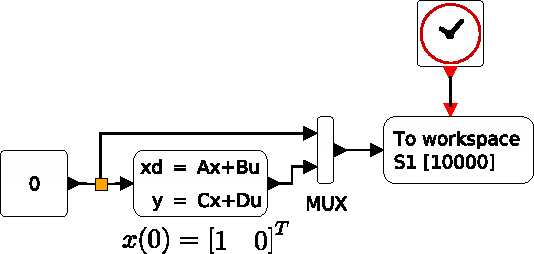
\includegraphics[width=250]{loop_co_sh.pdf}
		\caption{Схема моделирования замкнутой системы}
		\label{fg:loop_co_sh}
	\end{figure}

	\begin{figure}[h!]
		\centering
		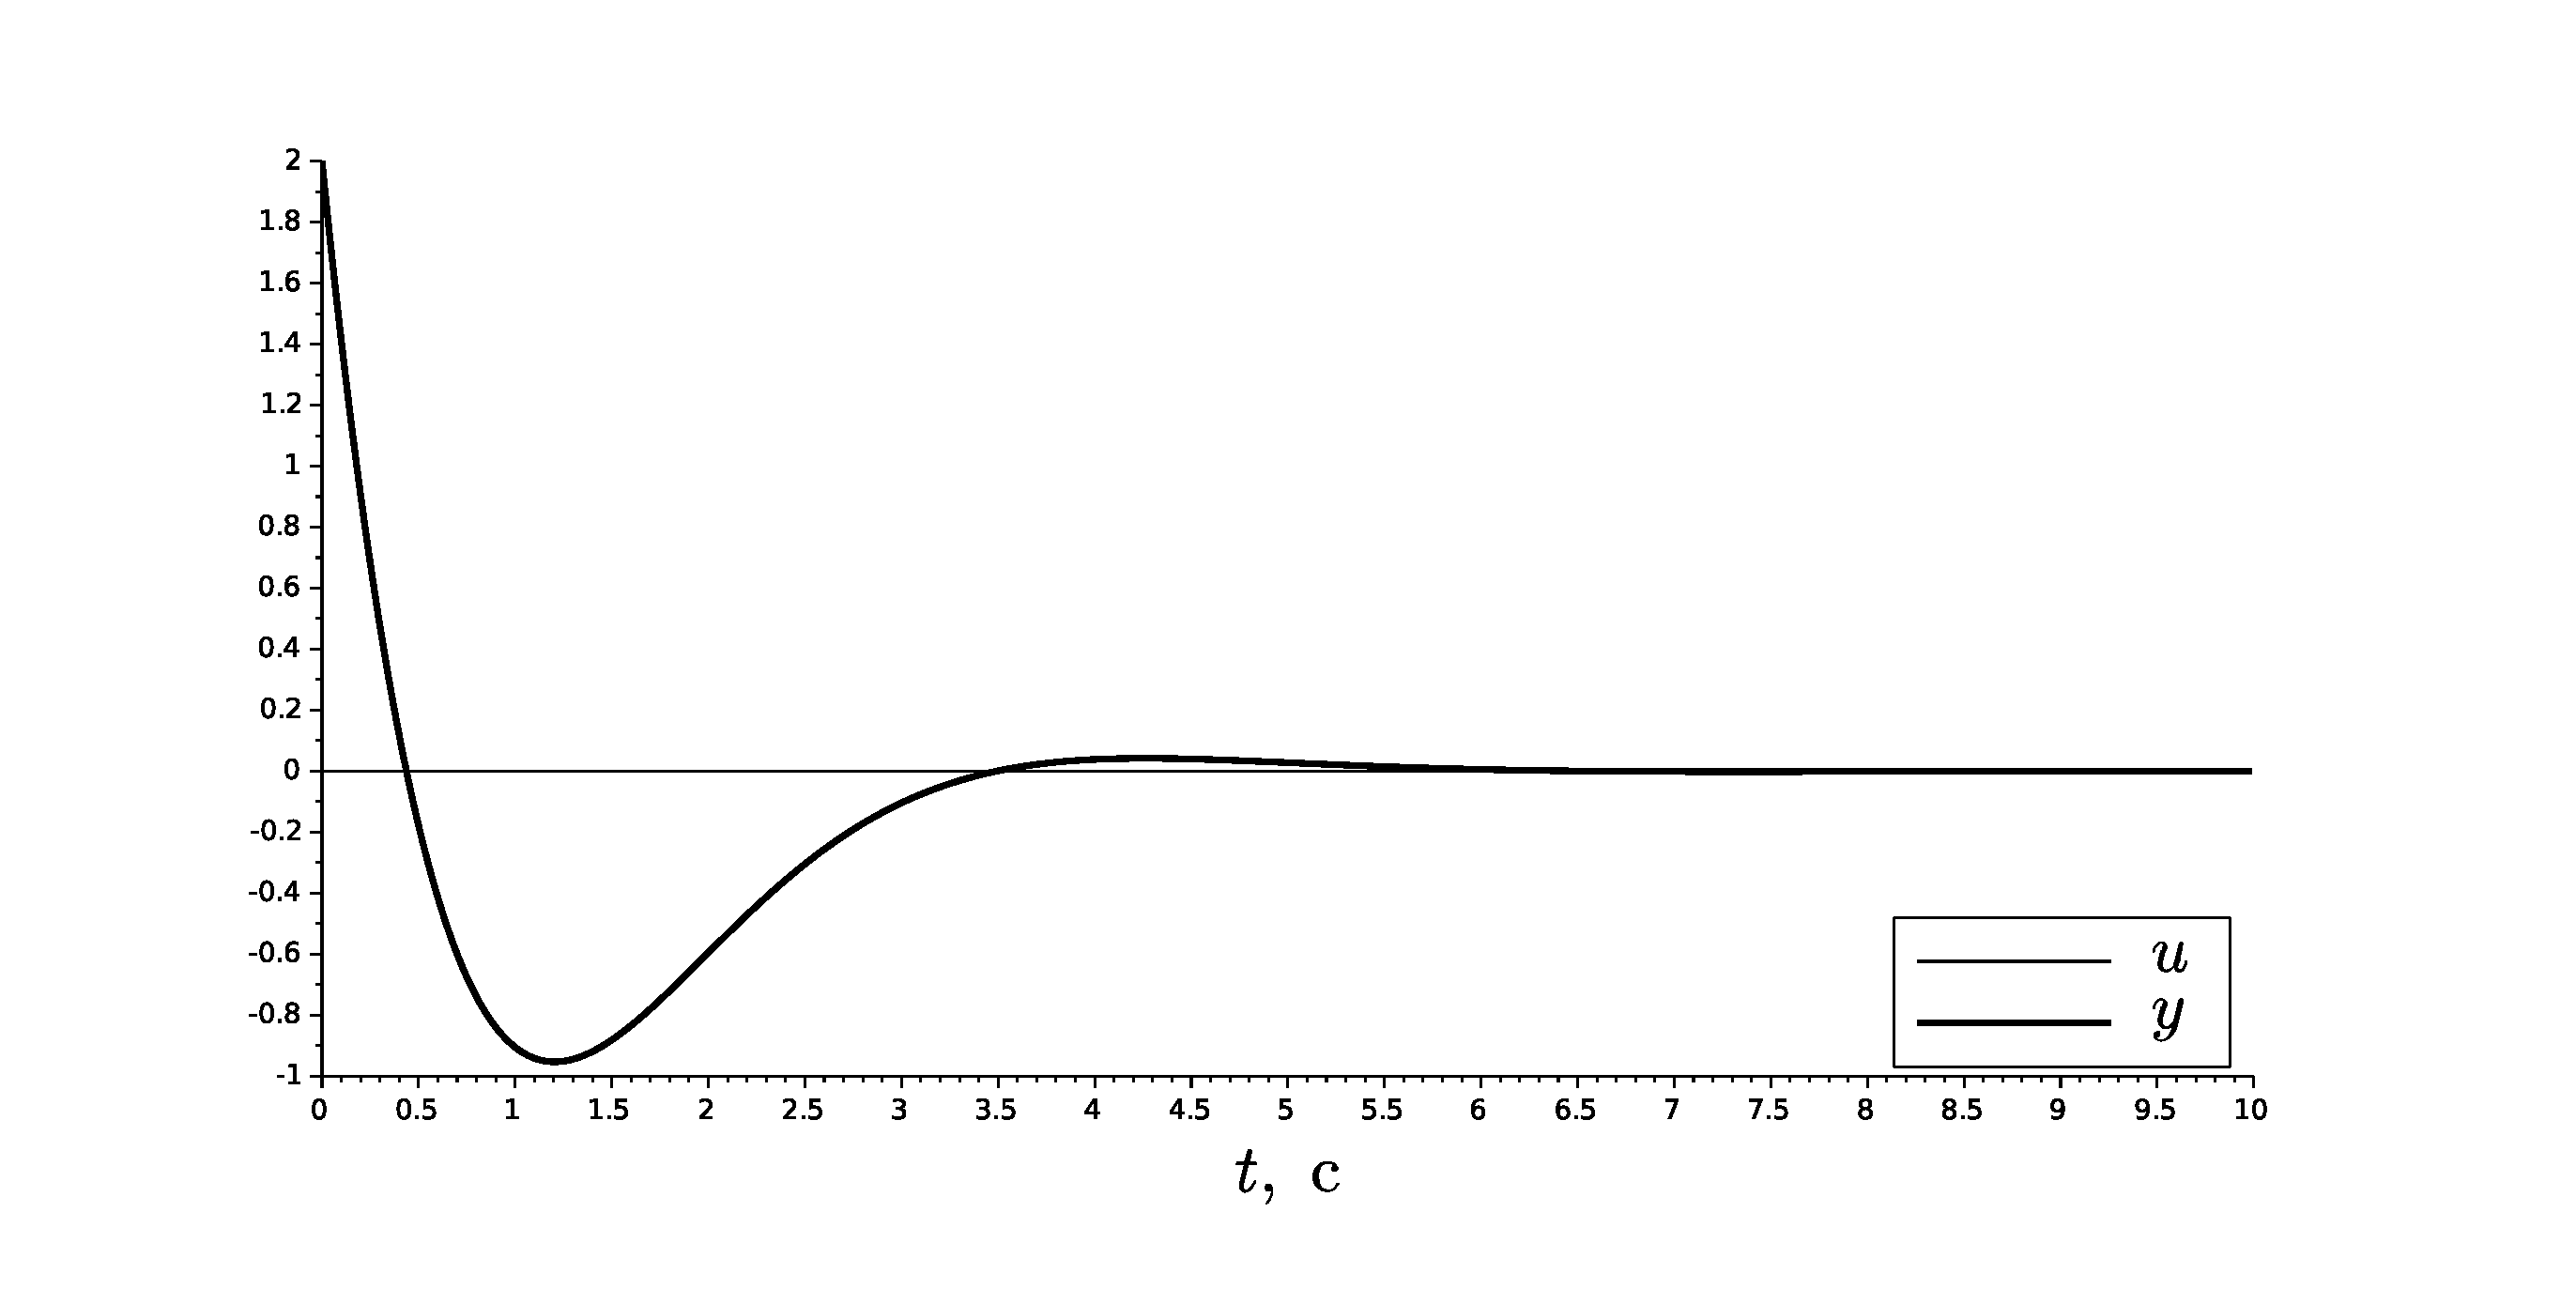
\includegraphics[width=\textwidth]{loop_co.pdf}
		\caption{Графики моделирования замкнутой системы при $x(0) = \begin{bmatrix} 1&0\end{bmatrix}^T$}
		\label{fg:loop_co}
	\end{figure}

	\item Полученная замкнутая система управления устойчива и обеспечивает заданные динамические показатели качества~\eqref{quality}.
\end{enumerate}

\subsection{Построение генератора сигнала задания}

Построим генератор сигналов в форме~\eqref{g_model}:

Для этого представим сигнал задания~\eqref{g} в виде суммы консервативного и пропорционального звеньев.

Модель консервативного звена в пространстве состояний:
\begin{equation}\label{g1}
	w_1 = g,~\dot{w}_1 = w_2,~\dot{w}_2 = - \omega_{g}^2 w_1  
\end{equation}
где начальные условия:
\begin{equation}
	w_1(0) = A_g,~w_2(0) = 0
\end{equation}

Модель пропорционального звена в пространстве состояния:
\begin{equation}\label{g2}
	w_3 = C_g,~\dot{w}_3 = 0
\end{equation}
где начальные условия
\begin{equation}
	w_3(0) = C_g
\end{equation}

Таким образом, матрица состояния генератора сигналов принимает вид:
\begin{equation}
	\Gamma = 
	\begin{bmatrix}
		0 & 1 & 0 \\
		-36 & 0 & 0 \\
		0 & 0 & 0
	\end{bmatrix}
\end{equation}

Матрица выхода:
\begin{equation}
	h = 
	\begin{bmatrix}
		1\\ 
		0\\
		1
	\end{bmatrix}
\end{equation}

Начальные условия:
\begin{equation}
	w(0) = 
	\begin{bmatrix}
		2\\
		0\\
		3
	\end{bmatrix}
\end{equation}

\begin{figure}[h!]
	\centering
	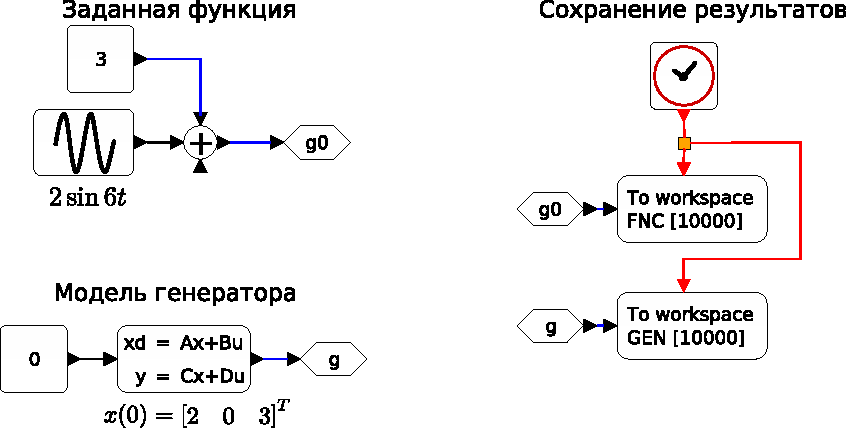
\includegraphics[width=300]{generator_sh.pdf}
	\caption{Схема моделирования генератора входного сигнала ($g$~--- генератор, $g0$~--- заданная функция)}
	\label{fg:generator_sh}
\end{figure}

\begin{figure}[h!]
	\centering
	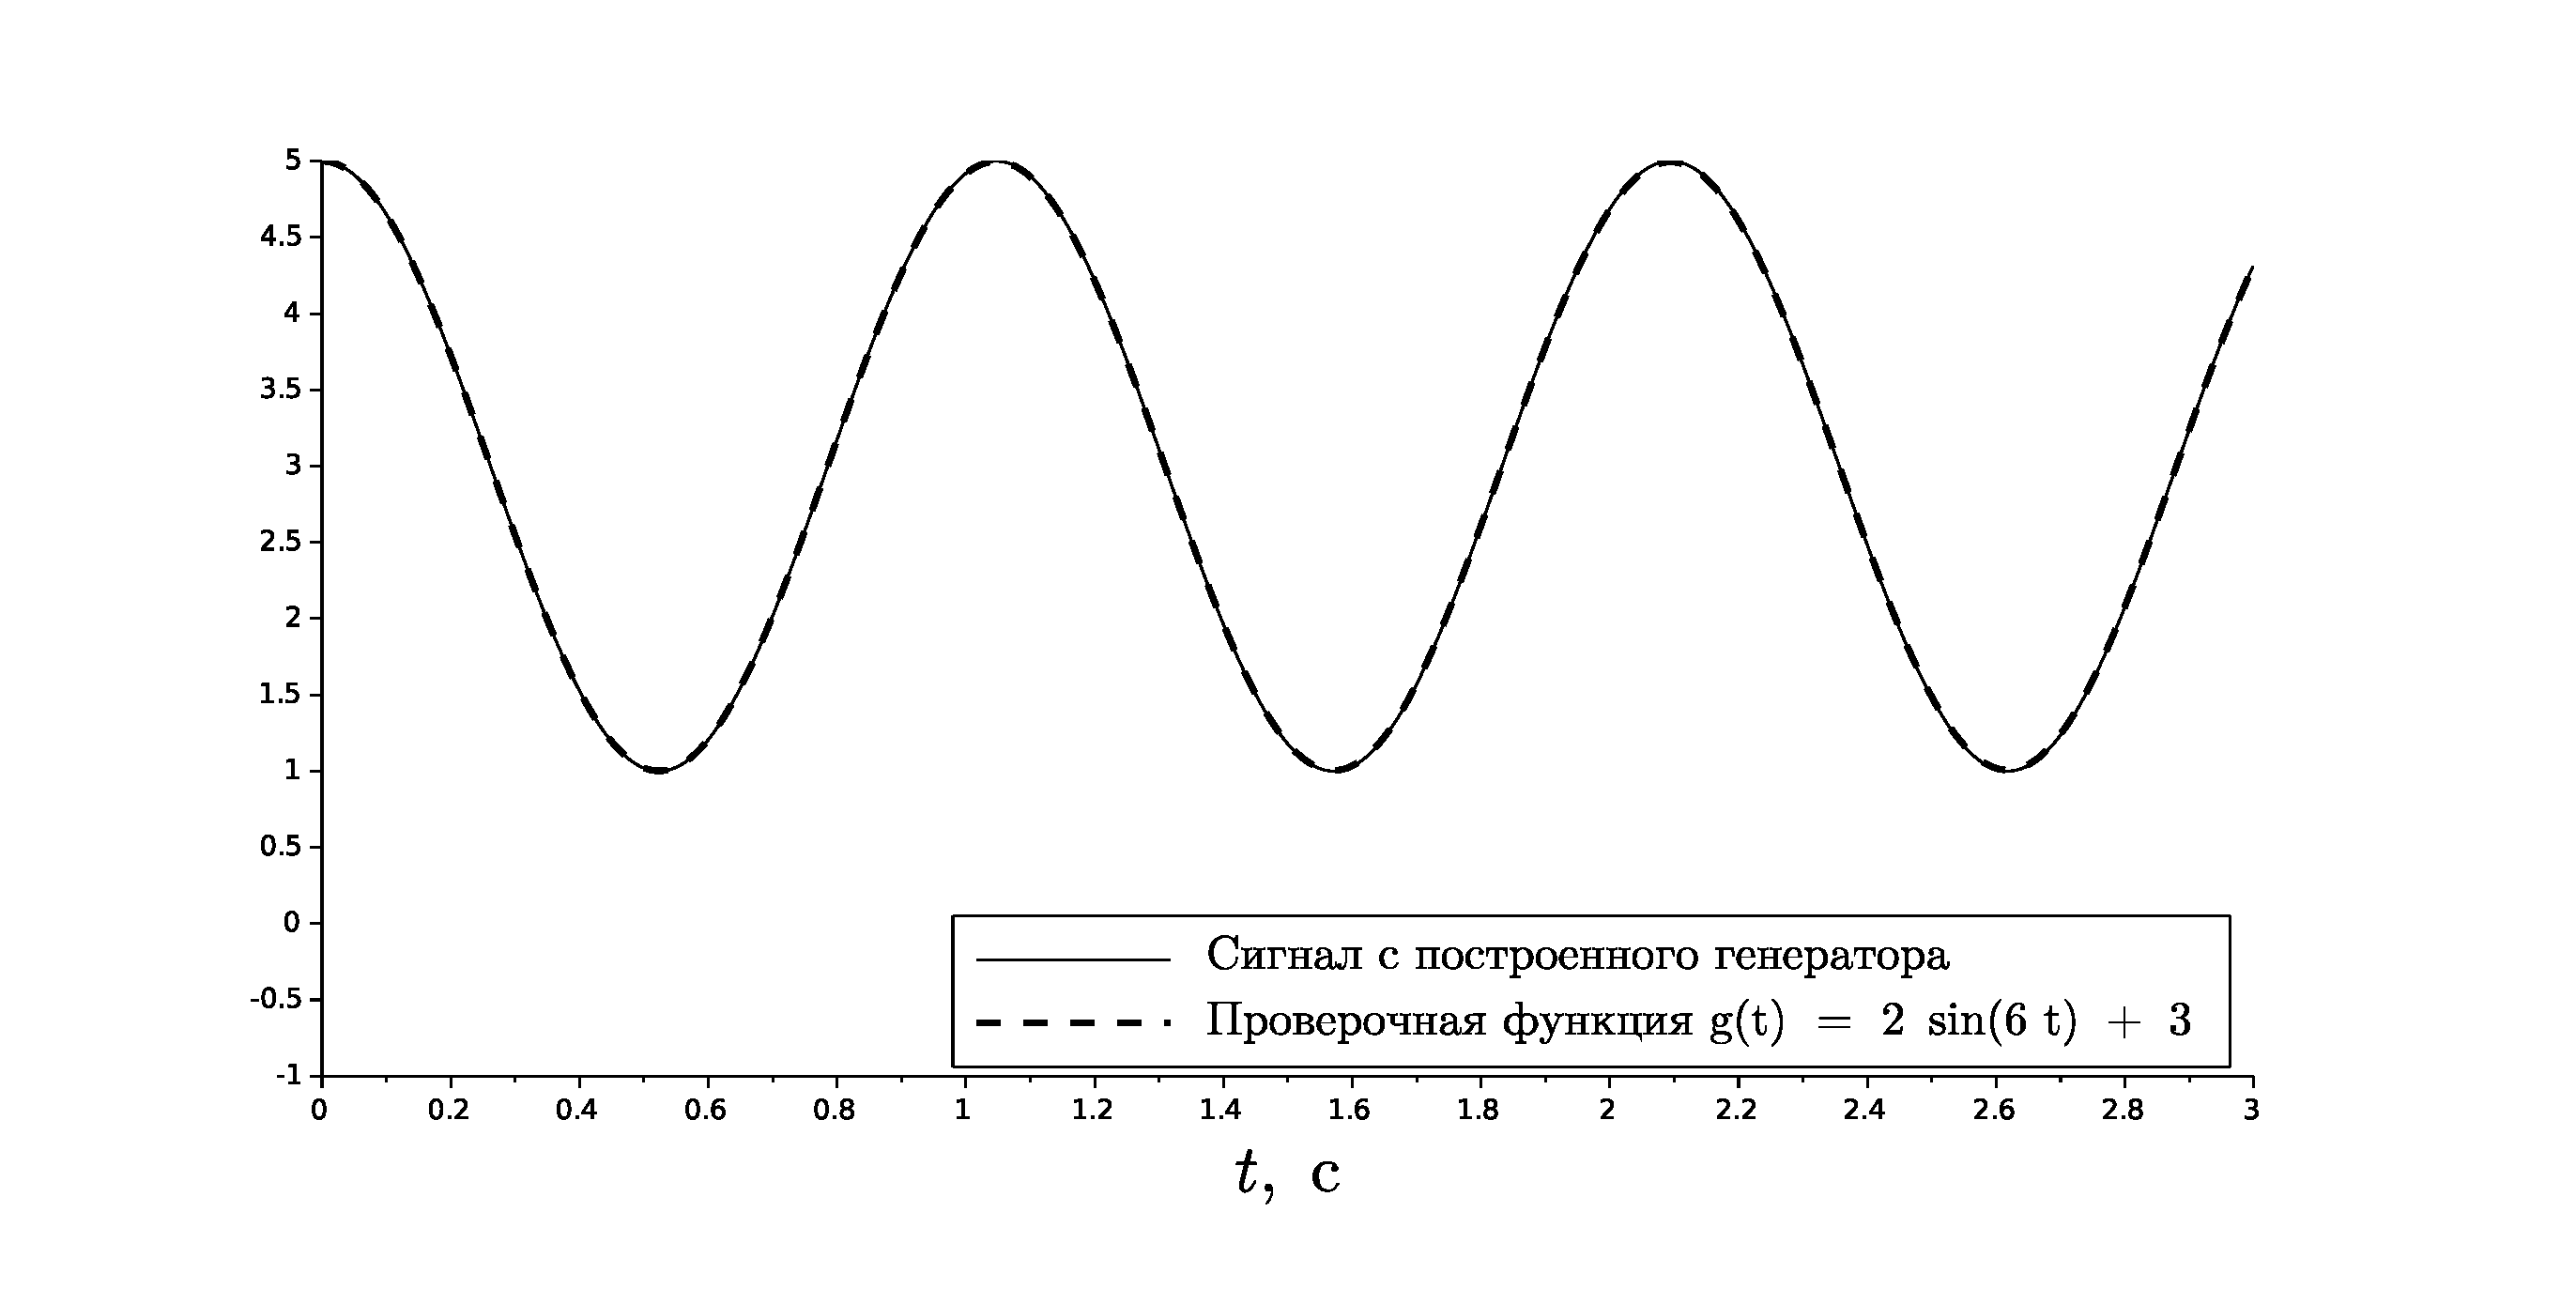
\includegraphics[width=450]{generator.pdf}
	\caption{Графики моделирования генератора входного сигнала}
	\label{fg:generator}
\end{figure}

\clearpage
\subsection{Построение параметризованной модели генератора задания}

Применим к уравнению~\eqref{g_model} матричную передаточную функцию~\eqref{pff}

Для обеспечения требуемых показателей качества в качестве характеристического полинома матрицы $\Gamma_0$ выбран стандартный полином Ньютона третьего порядка
\begin{equation}
(\lambda + \omega_0)^3 = \lambda^3 +  3 \omega_0 \lambda^2 + 3 \omega_0^2 \lambda + \omega_0^3,
\end{equation}
где
\begin{equation}
\omega_0 = \frac{6.3}{t_\text{п}} = \frac{6.3}{3} = 2.1,
\end{equation}
где, в свою очередь, $6.3$~с~--- стандартное время переходного процесса, а $t_\text{п}$~--- задано в~\eqref{filter_quality}.


Итого, матрица~$\Gamma_0$ имеет следующий вид
\begin{equation}
	\Gamma_0 =
	\begin{bmatrix}
		-6.3 & 1 & 0 \\
		-13.23 & 0 & 1 \\
		-9.261 & 0 & 0
	\end{bmatrix}
\end{equation}

После преобразований, получим:
\begin{gather}
	\Phi(s) [\dot{w}] = \Phi(s) \Gamma [w], \\
	%
	\Phi(s) (sI \pm \Gamma_0) [w] = \Phi(s) \Gamma [w], \\ 
	%
	w = \Phi(s) (\Gamma - \Gamma_0) [w], \\
	%
	w = \Phi(s) 
	\begin{bmatrix}
	k_2 \\ k_1 - \omega_g^2 \\ k_0        
	\end{bmatrix}
	[g] \\
	%
	g = \sum_{i=1}^{3} \theta_{i} \underbrace{C_{\xi} \Phi(s) e_{i} [g]}_{\xi_i} =  \theta^T \xi,
\end{gather}
где $e_i^T = [0\;0\;\ldots\;0\;\underbrace{1}_{i-th}\;0\;\ldots\;0]$, $C_{\xi} = [1\;0\;0]$.


\begin{figure}[h!]
	\centering
	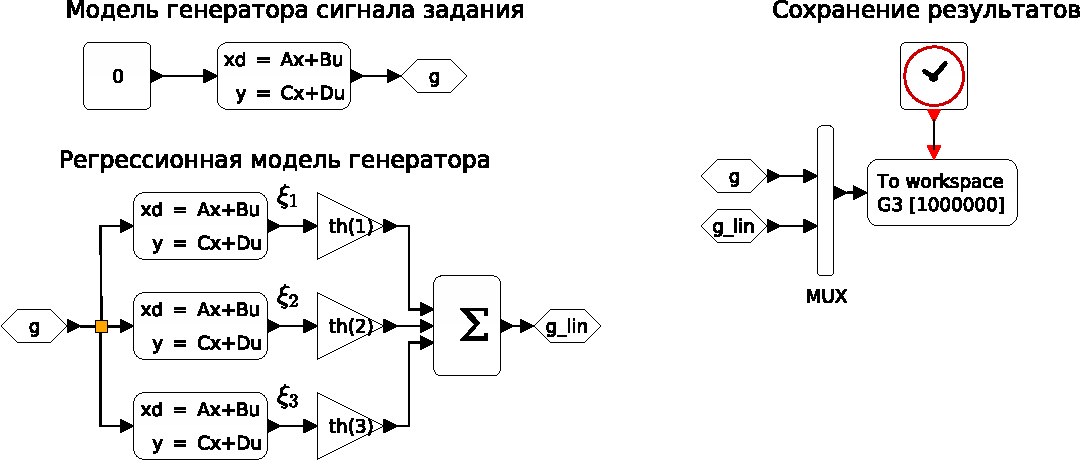
\includegraphics[width=500]{generator_parametric_sh.pdf}
	\caption{Схема моделирования параметризованной модели генератора входного сигнала}
	\label{fg:generator_parametric_sh}
\end{figure}

\begin{figure}[h!]
	\centering
	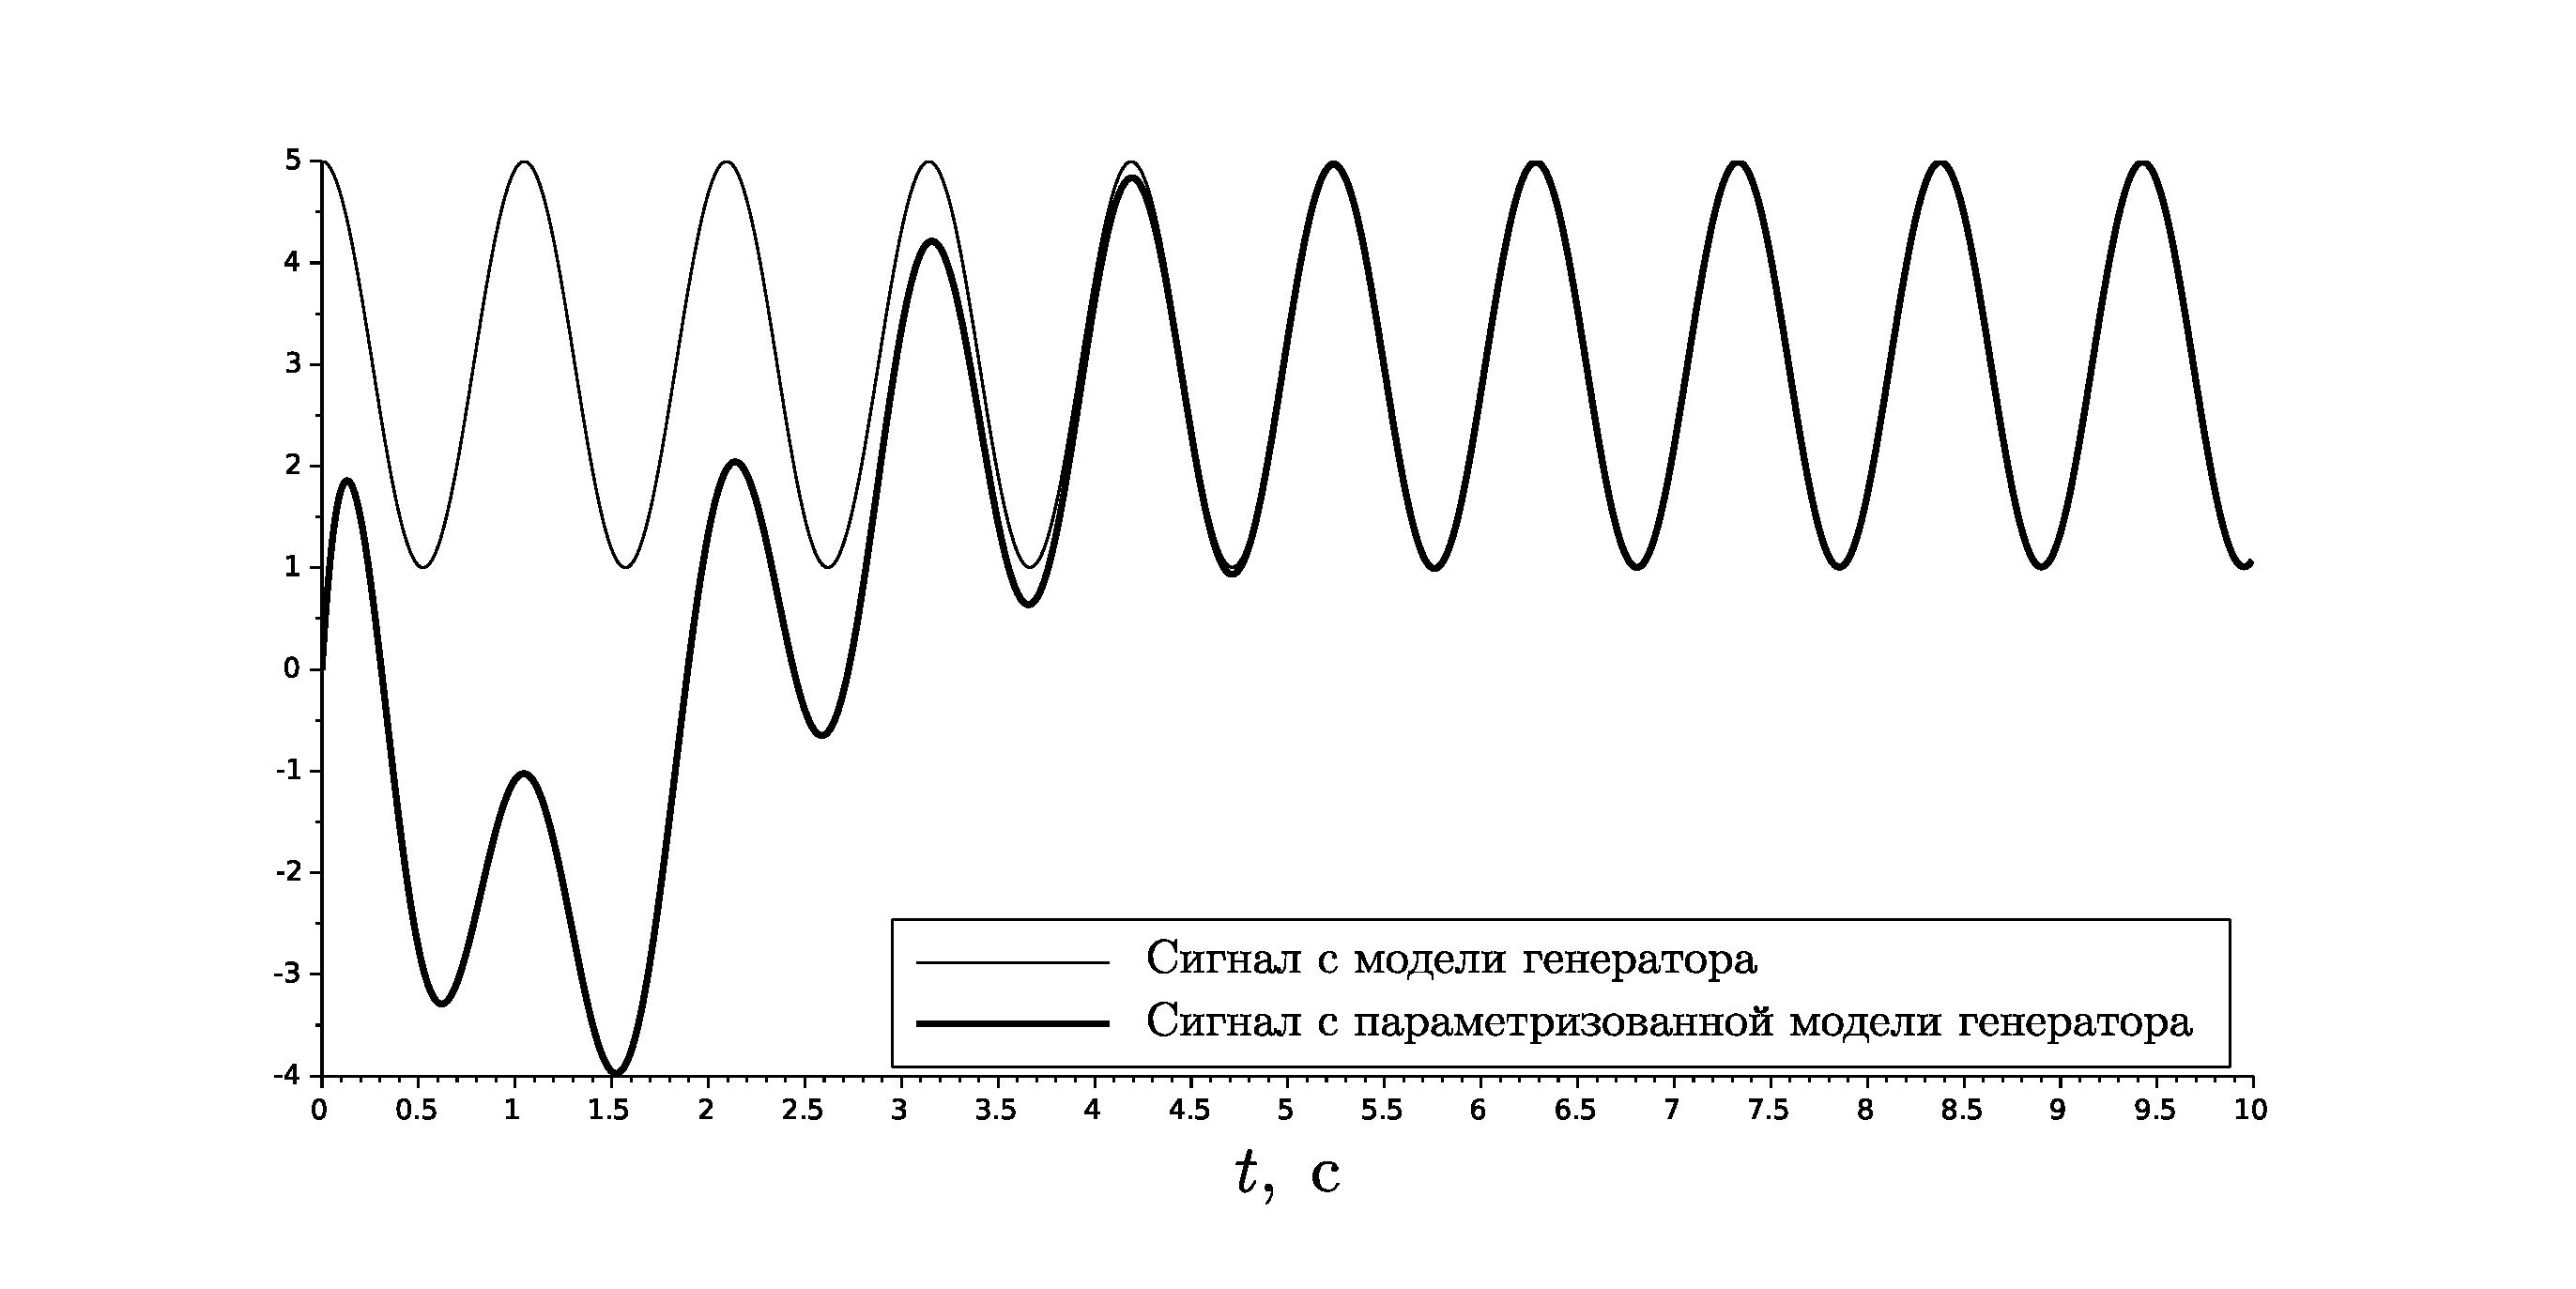
\includegraphics[width=\textwidth]{generator_parametric.pdf}
	\caption{Графики моделирования параметризованного генератора входного сигнала}
	\label{fg:generator_parametric}
\end{figure}

\clearpage
\subsection{Построение адаптивного идентификатора параметров модели задающего сигнала}

Заменим параметры $\theta$ на их оценки $\hat{\theta}$ и сформируем модель генератора в виде:
\begin{equation}
	\hat{g} = \hat{\theta}^T \xi,
\end{equation}
где $\hat{g}$~--- оценка переменной $g$.

Введем в рассмотрение ошибку:
\begin{equation}
	\tilde{g} = g - \hat{g}
\end{equation}
После преобразований, получим
\begin{equation}
	\tilde{g} = \tilde{\theta}^t \xi
\end{equation}

Алгоритм адаптации:
\begin{equation}
	\dot{\hat{\theta}} = \gamma \xi \varepsilon
\end{equation}
где $\gamma > 0$~--- коэффициент адаптации.

\begin{figure}[h!]
	\centering
	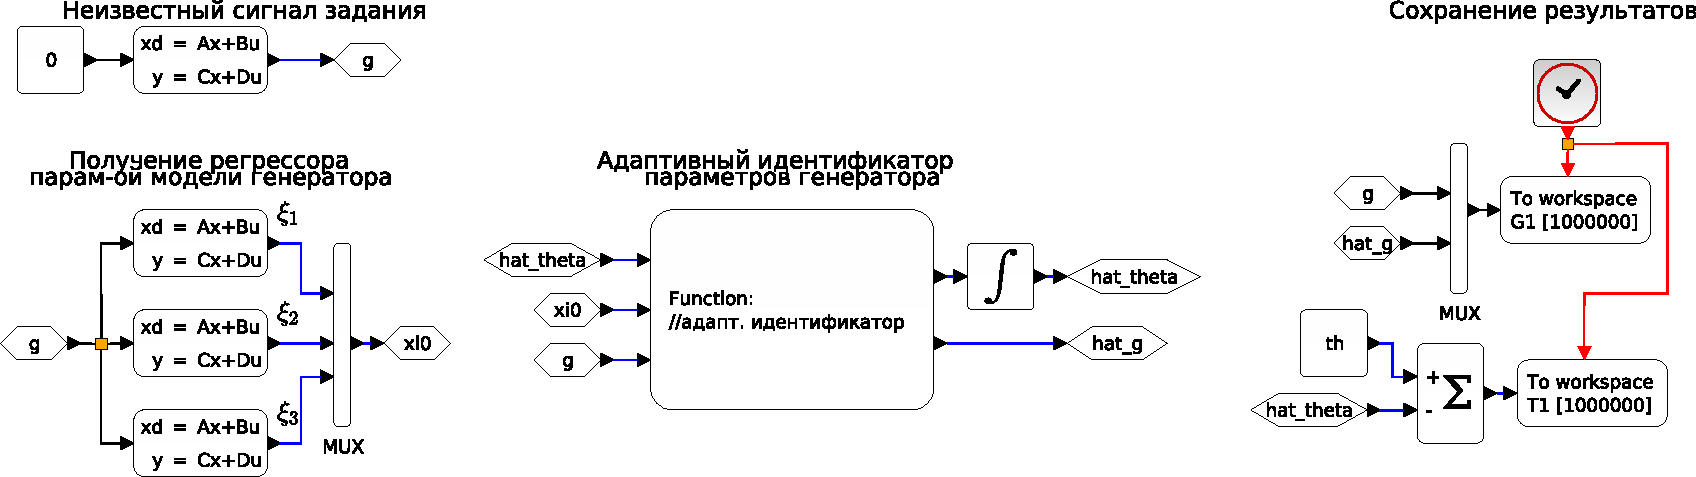
\includegraphics[width=500]{generator_parametric_adpt_g_sh.pdf}
	\caption{Схема моделирования идентификатора параметров генератора}
	\label{fg:generator_parametric_adapt_sh}
\end{figure}

\begin{figure}[h!]
	\centering
	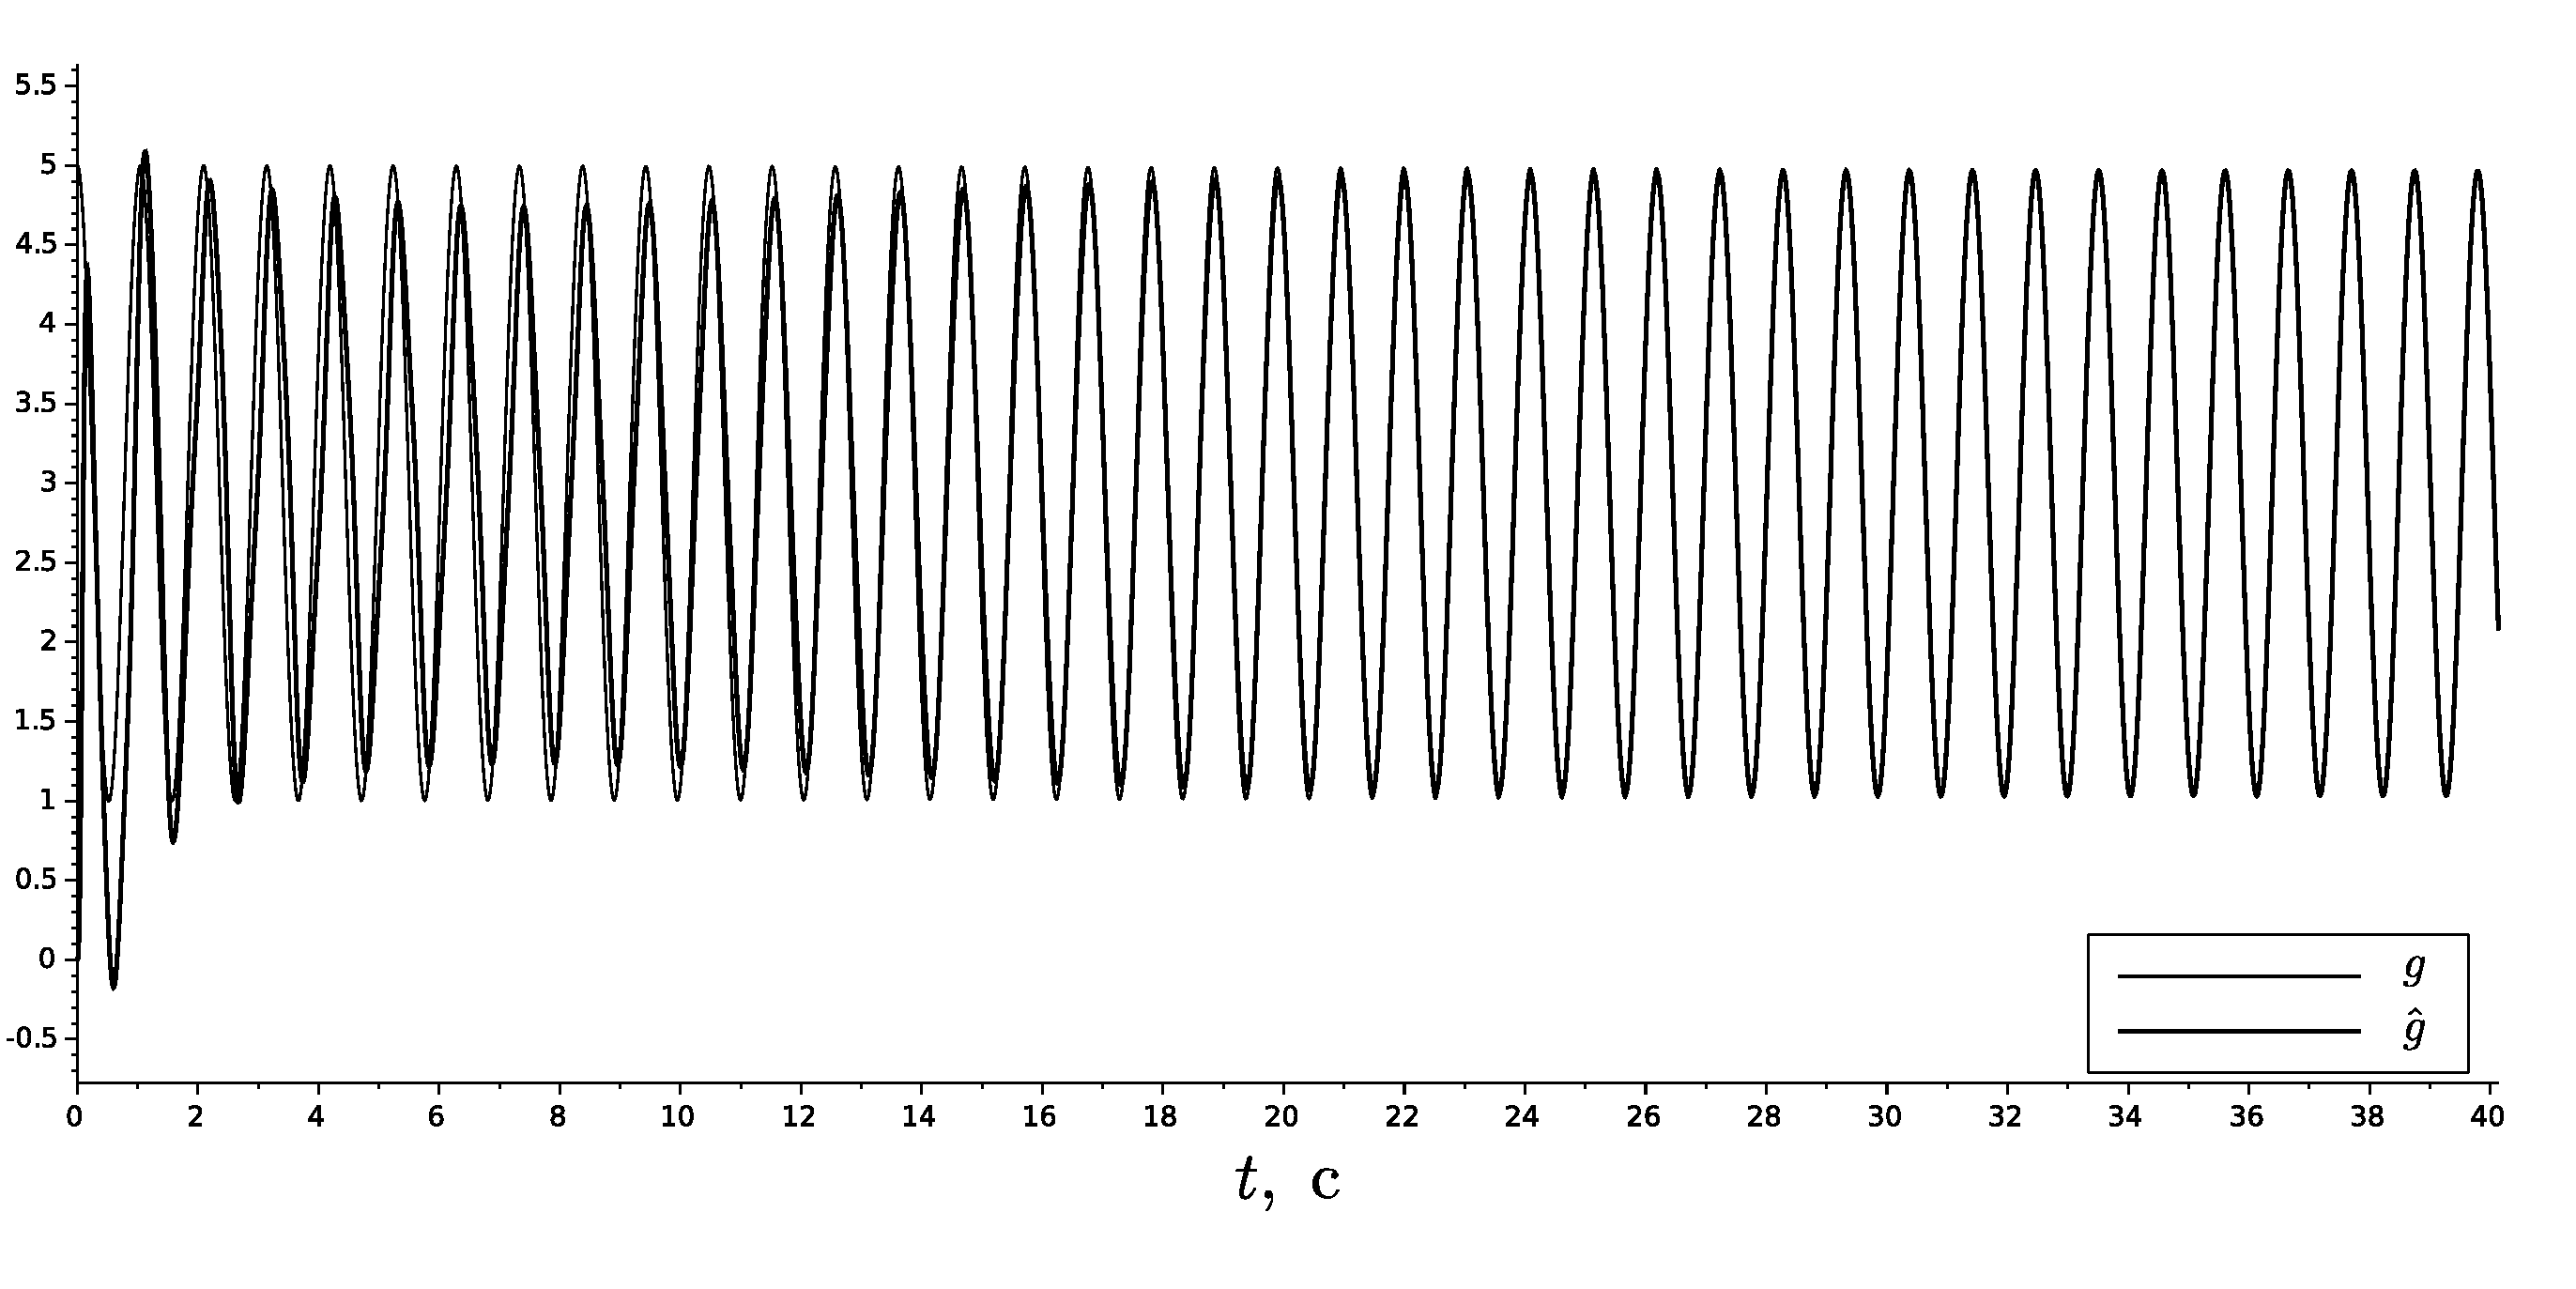
\includegraphics[width=\textwidth]{generator_parametric_adpt_g_signals.pdf}
	\caption{Графики, изображающие выходные сигнала генератора и и его оценки, $\gamma = 120$}
	\label{fg:generator_parametric_adapt_signals}
\end{figure}

\begin{figure}[h!]
	\centering
	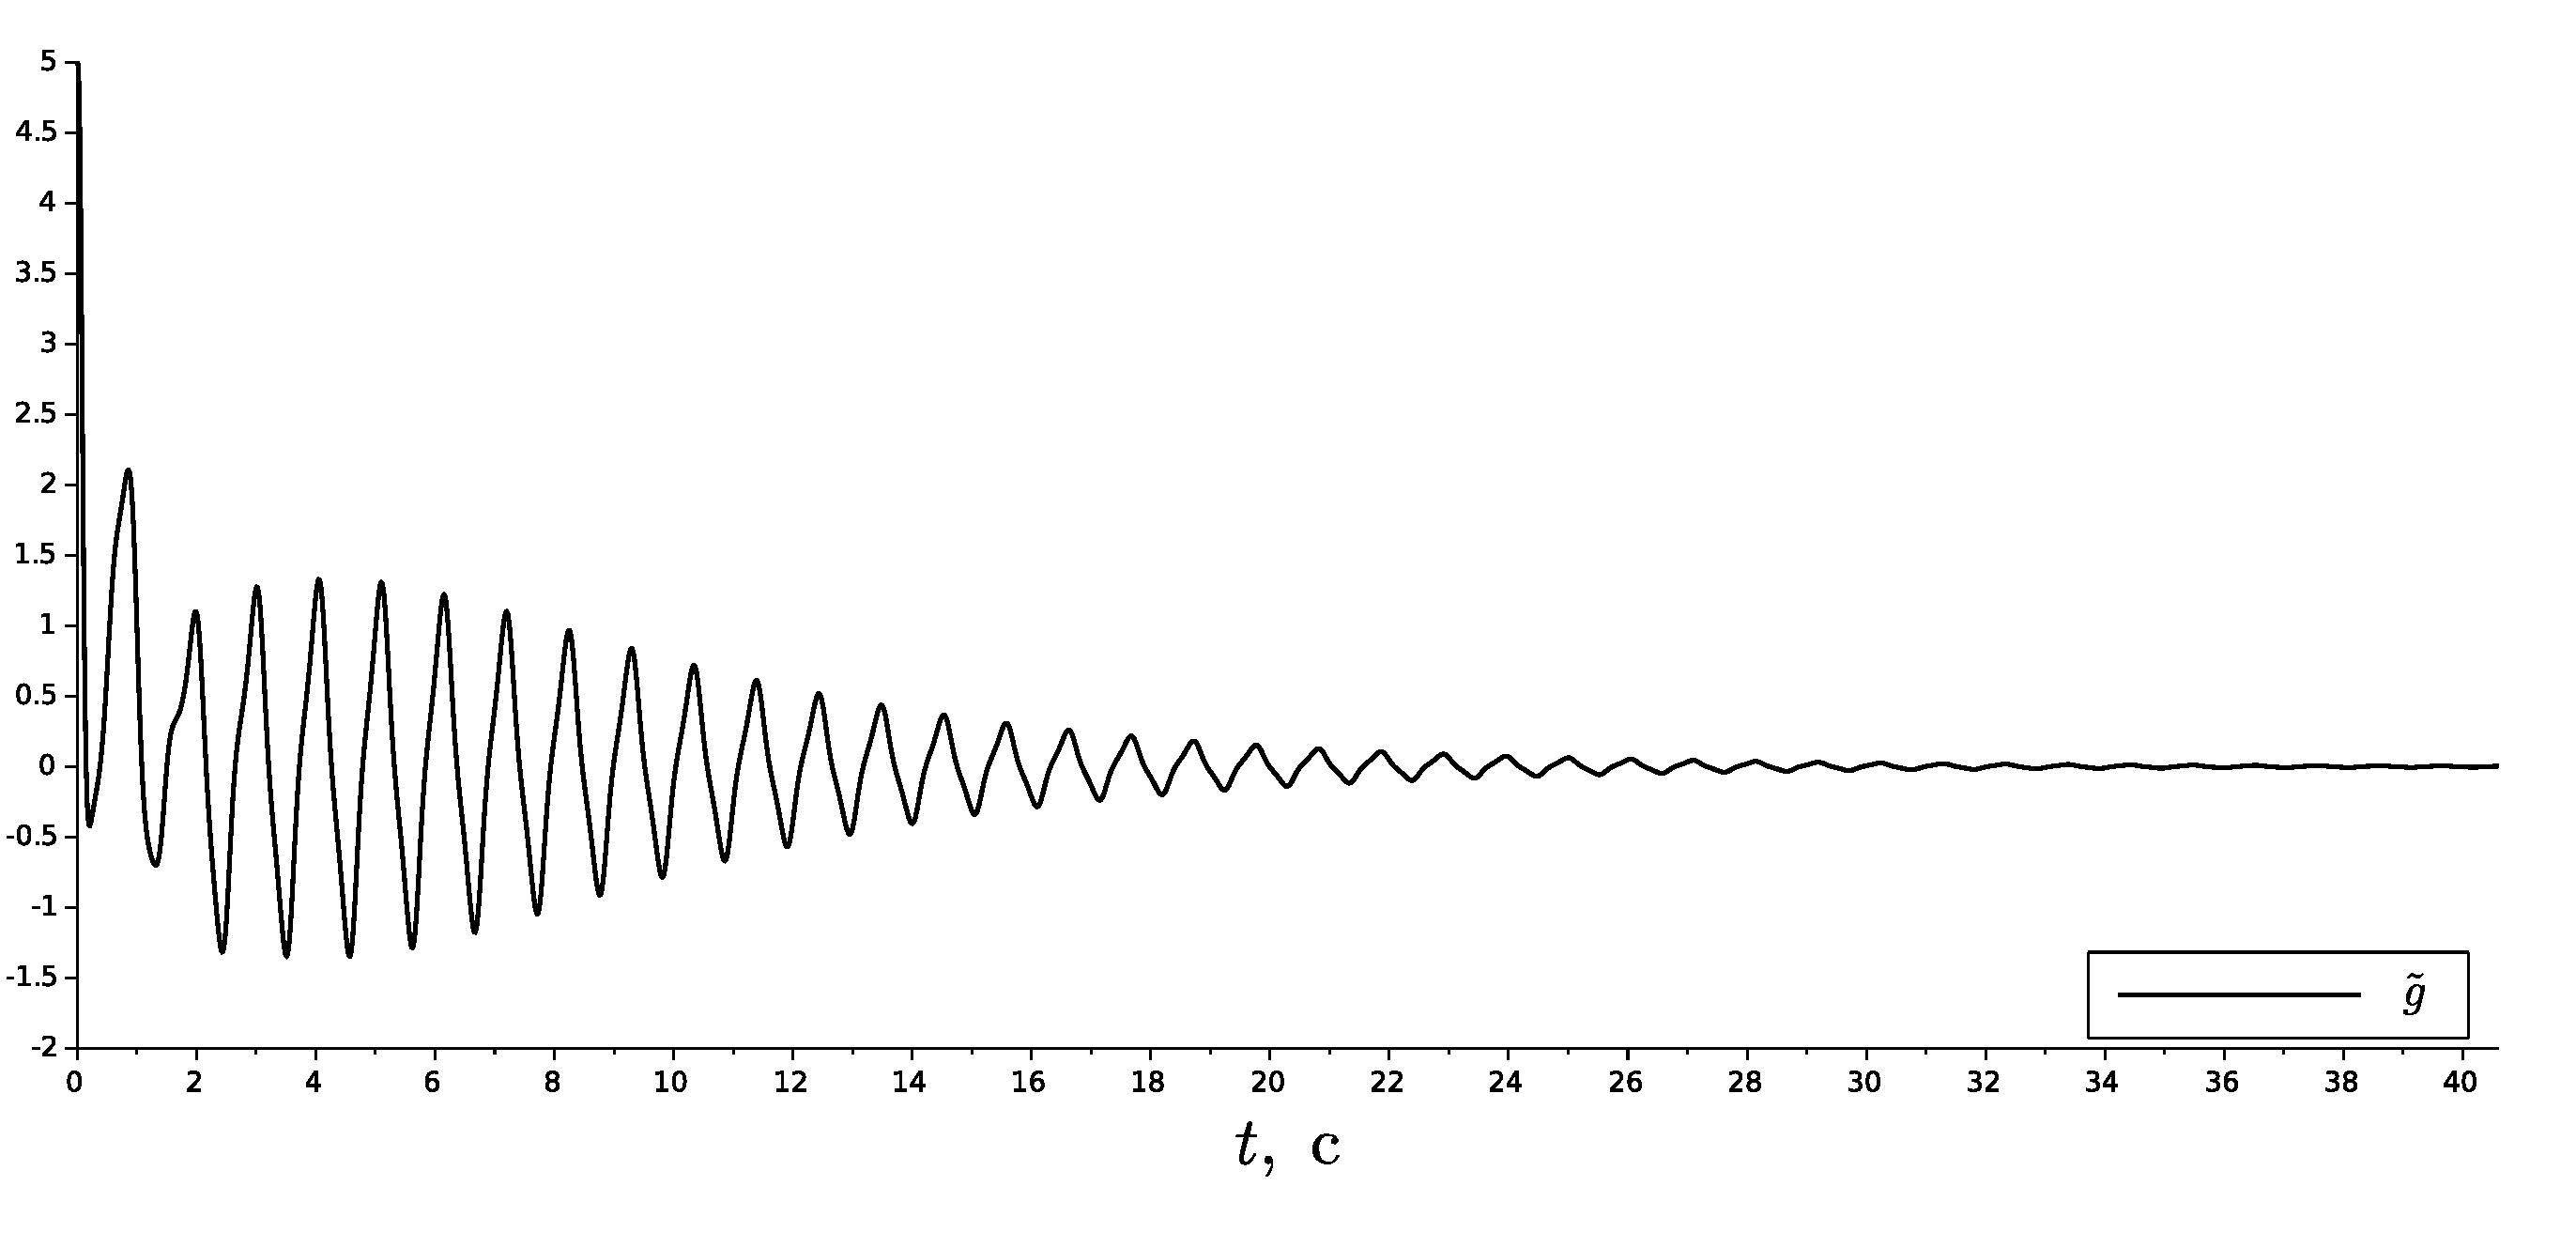
\includegraphics[width=\textwidth]{generator_parametric_adpt_g.pdf}
	\caption{Графики, изображающие ошибку выходной переменной генератора задающего сигнала во время идентификации его параметров}
	\label{fg:generator_parametric_adapt}
\end{figure}
\clearpage
\begin{figure}[h!]
	\centering
	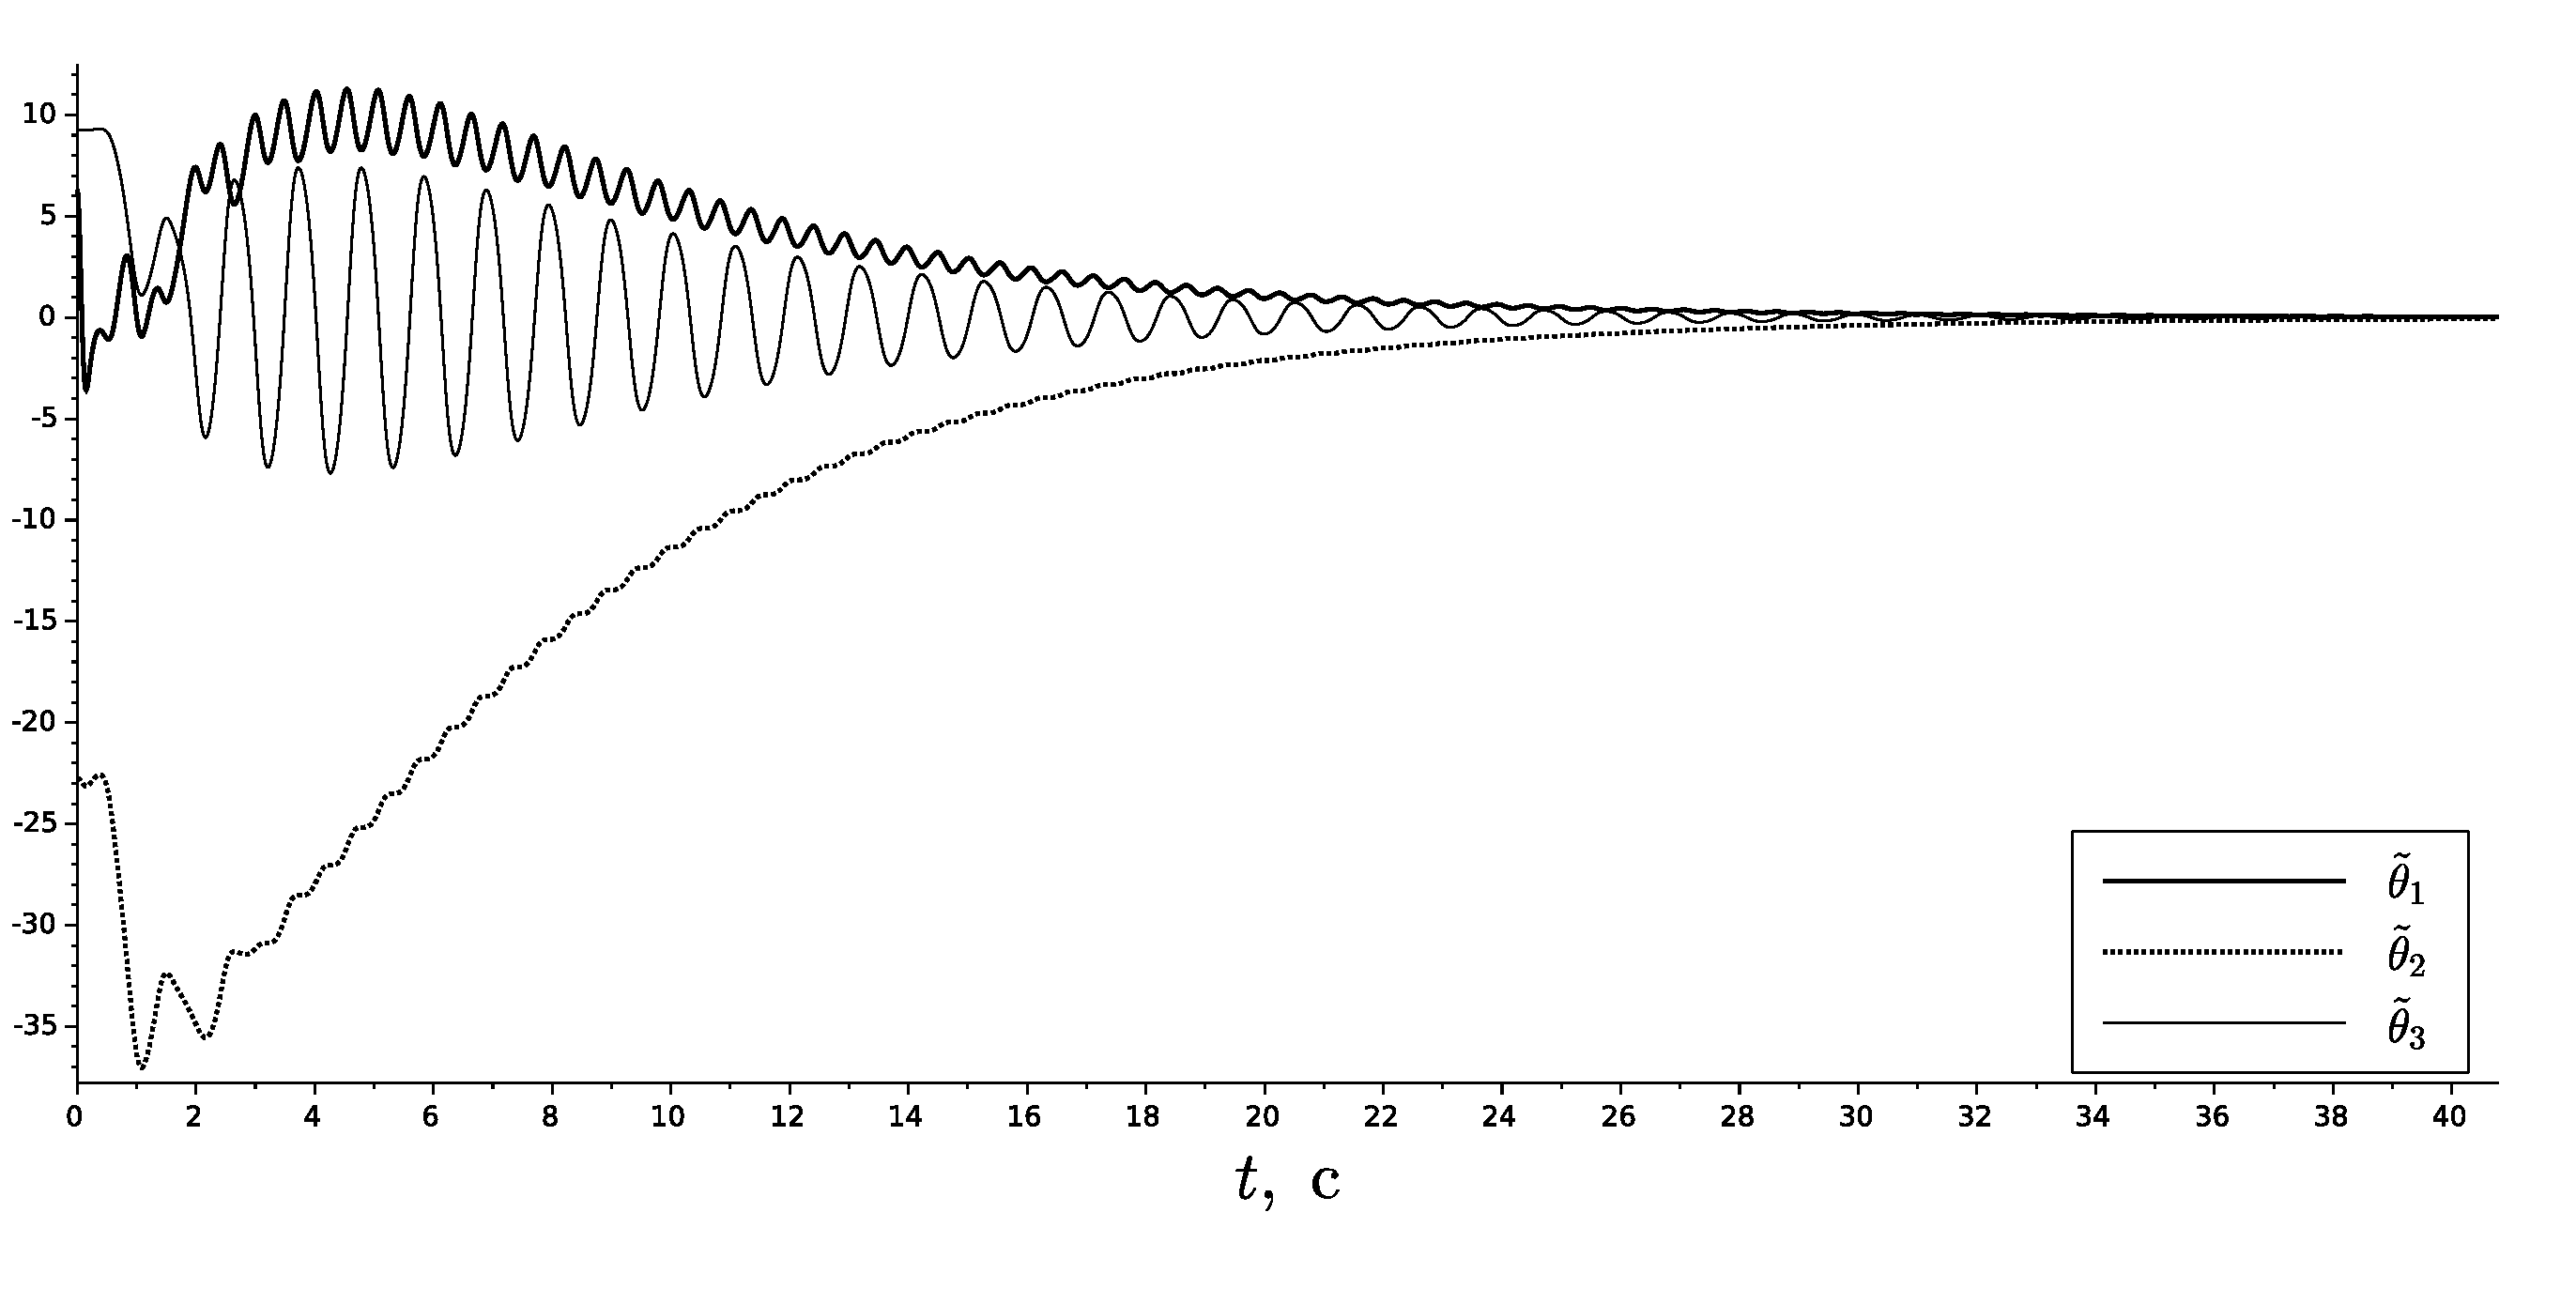
\includegraphics[width=\textwidth]{tilde_theta.pdf}
	\caption{Графики, изображающие ошибку вектора параметров генератора ЗВ}
	\label{fg:generator_parametric_adapt_theta}
\end{figure}


\subsection{Реализация адаптивного алгоритма слежения из п 3.3}

\begin{figure}[h!]
	\centering
	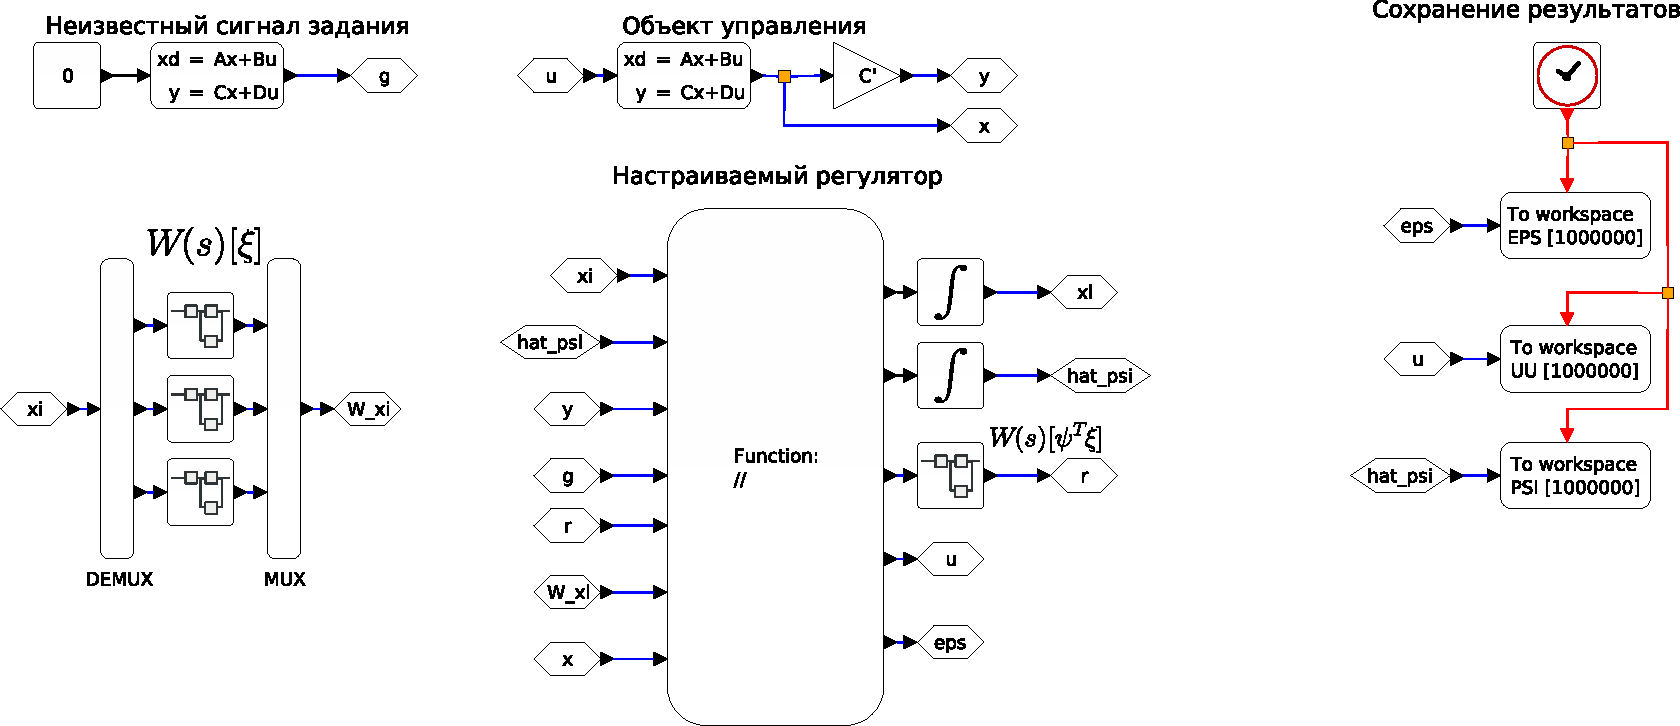
\includegraphics[width=500]{fin_sh.pdf}
	\caption{Схема моделирования системы слежения}
	\label{fg:fin}
\end{figure}

\begin{figure}[h!]
	\centering
	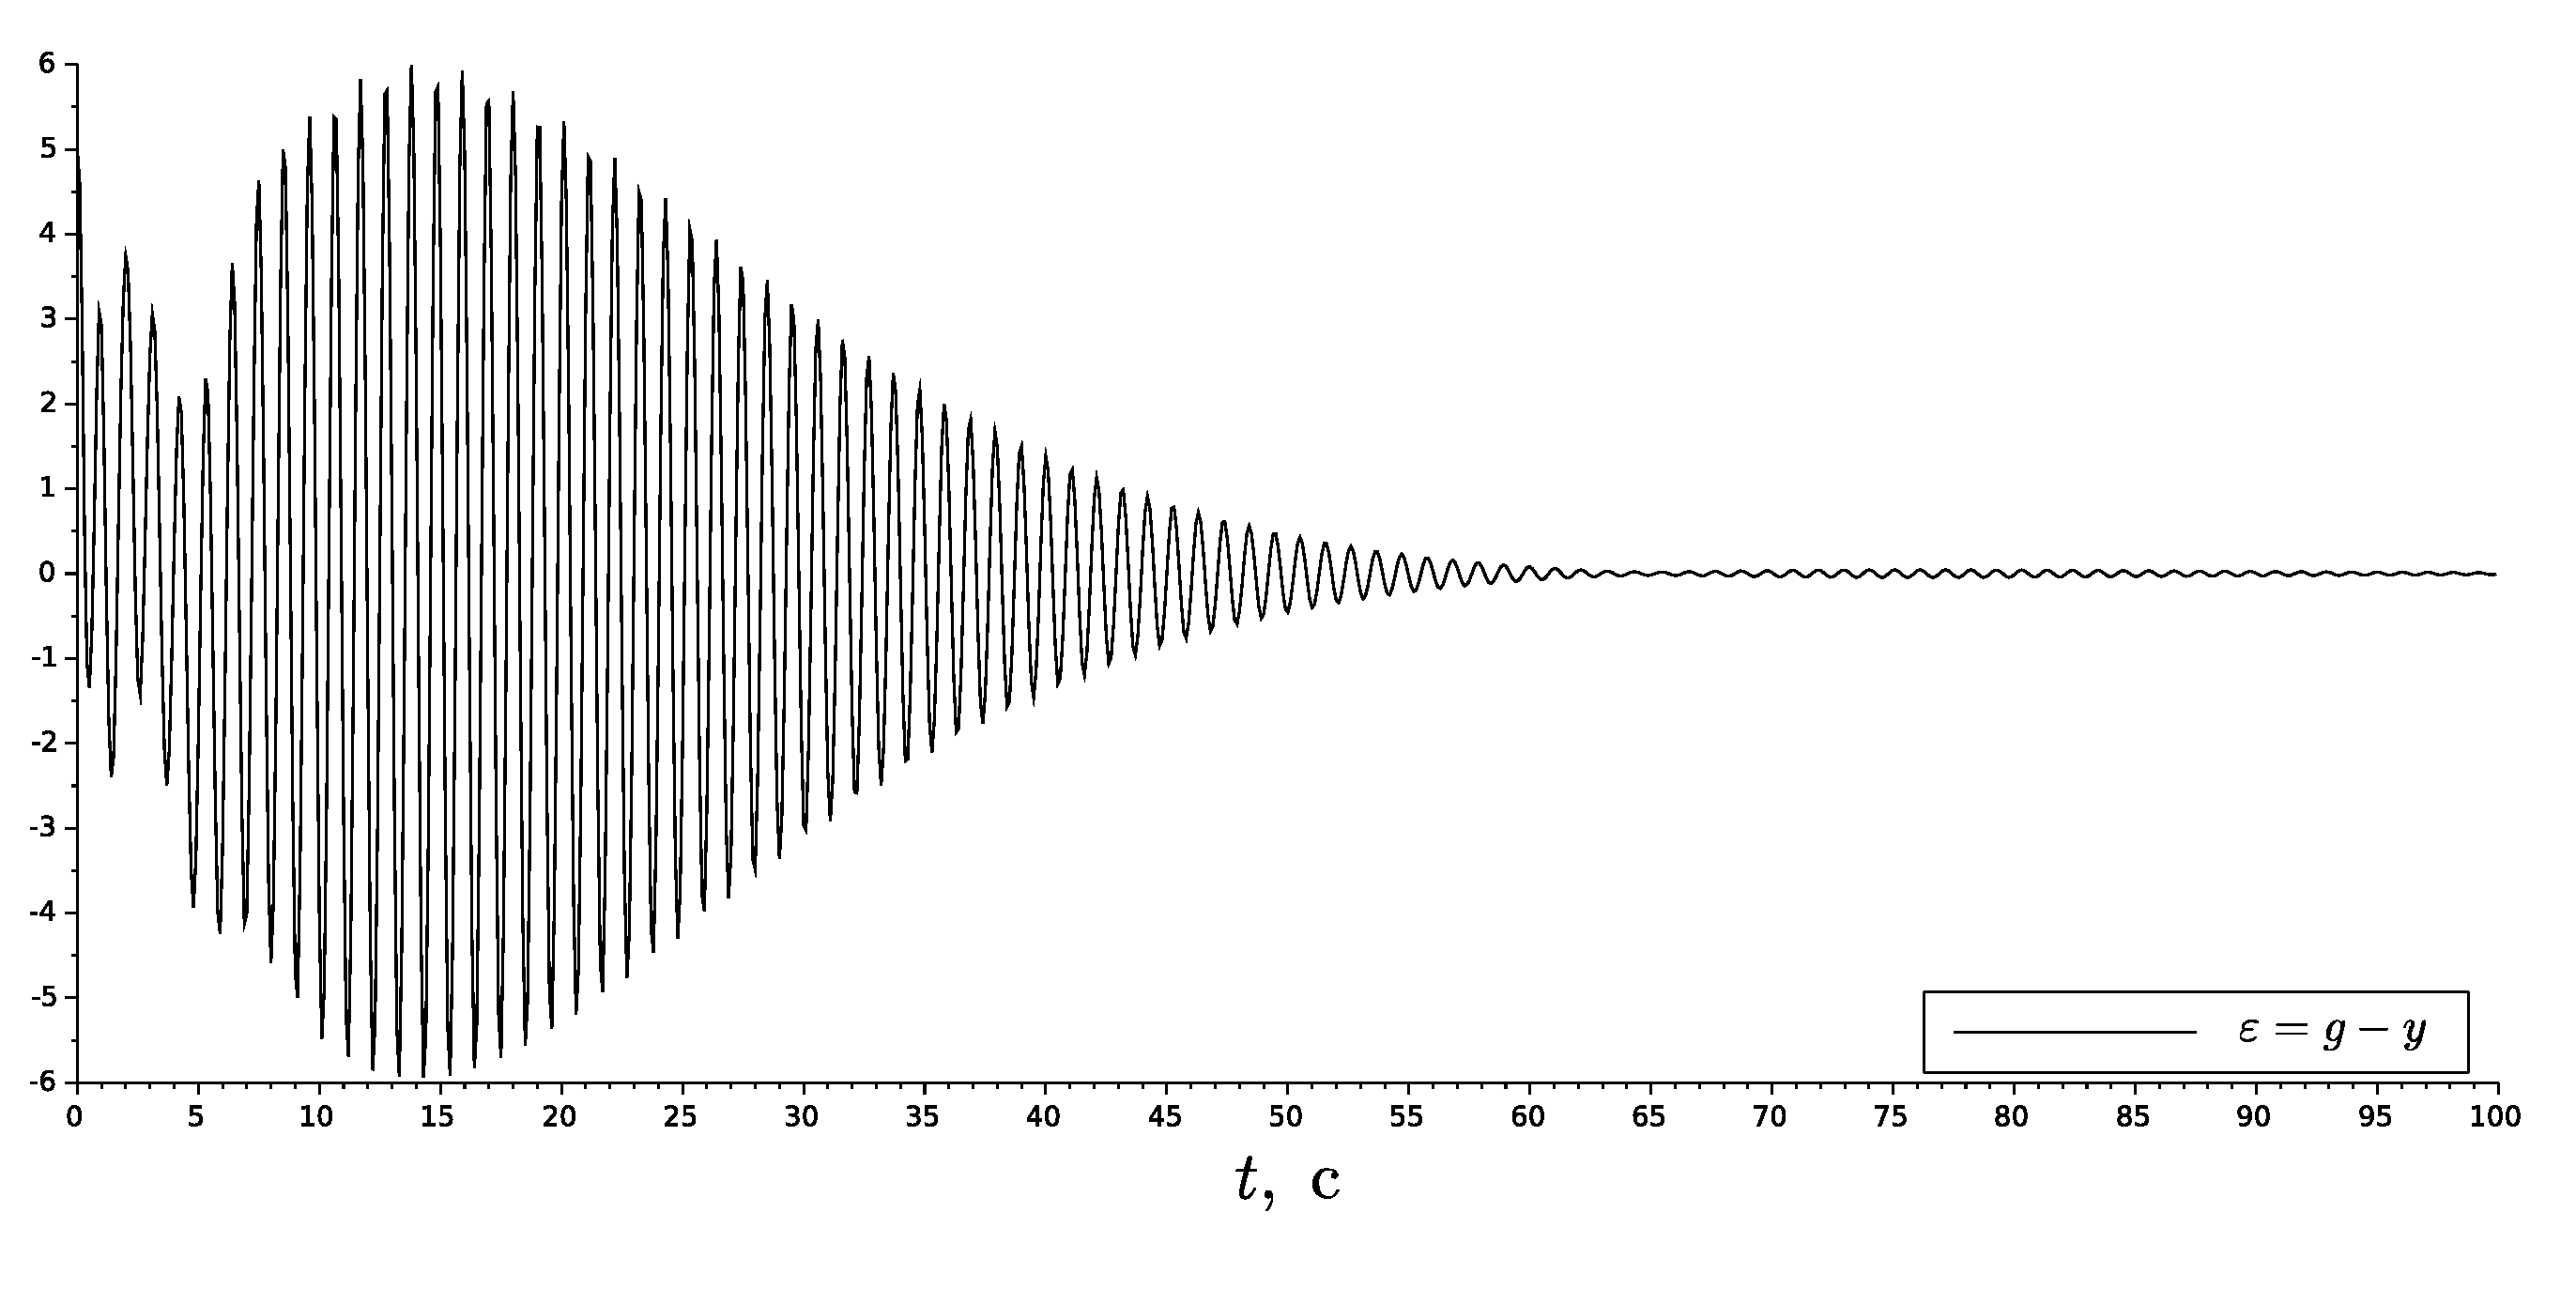
\includegraphics[width=\textwidth]{vareps.pdf}
	\caption{Графики, изображающие ошибку $\varepsilon = g - y$, $\gamma = 13$}
	\label{fg:fin_}
\end{figure}

\begin{figure}[h!]
	\centering
	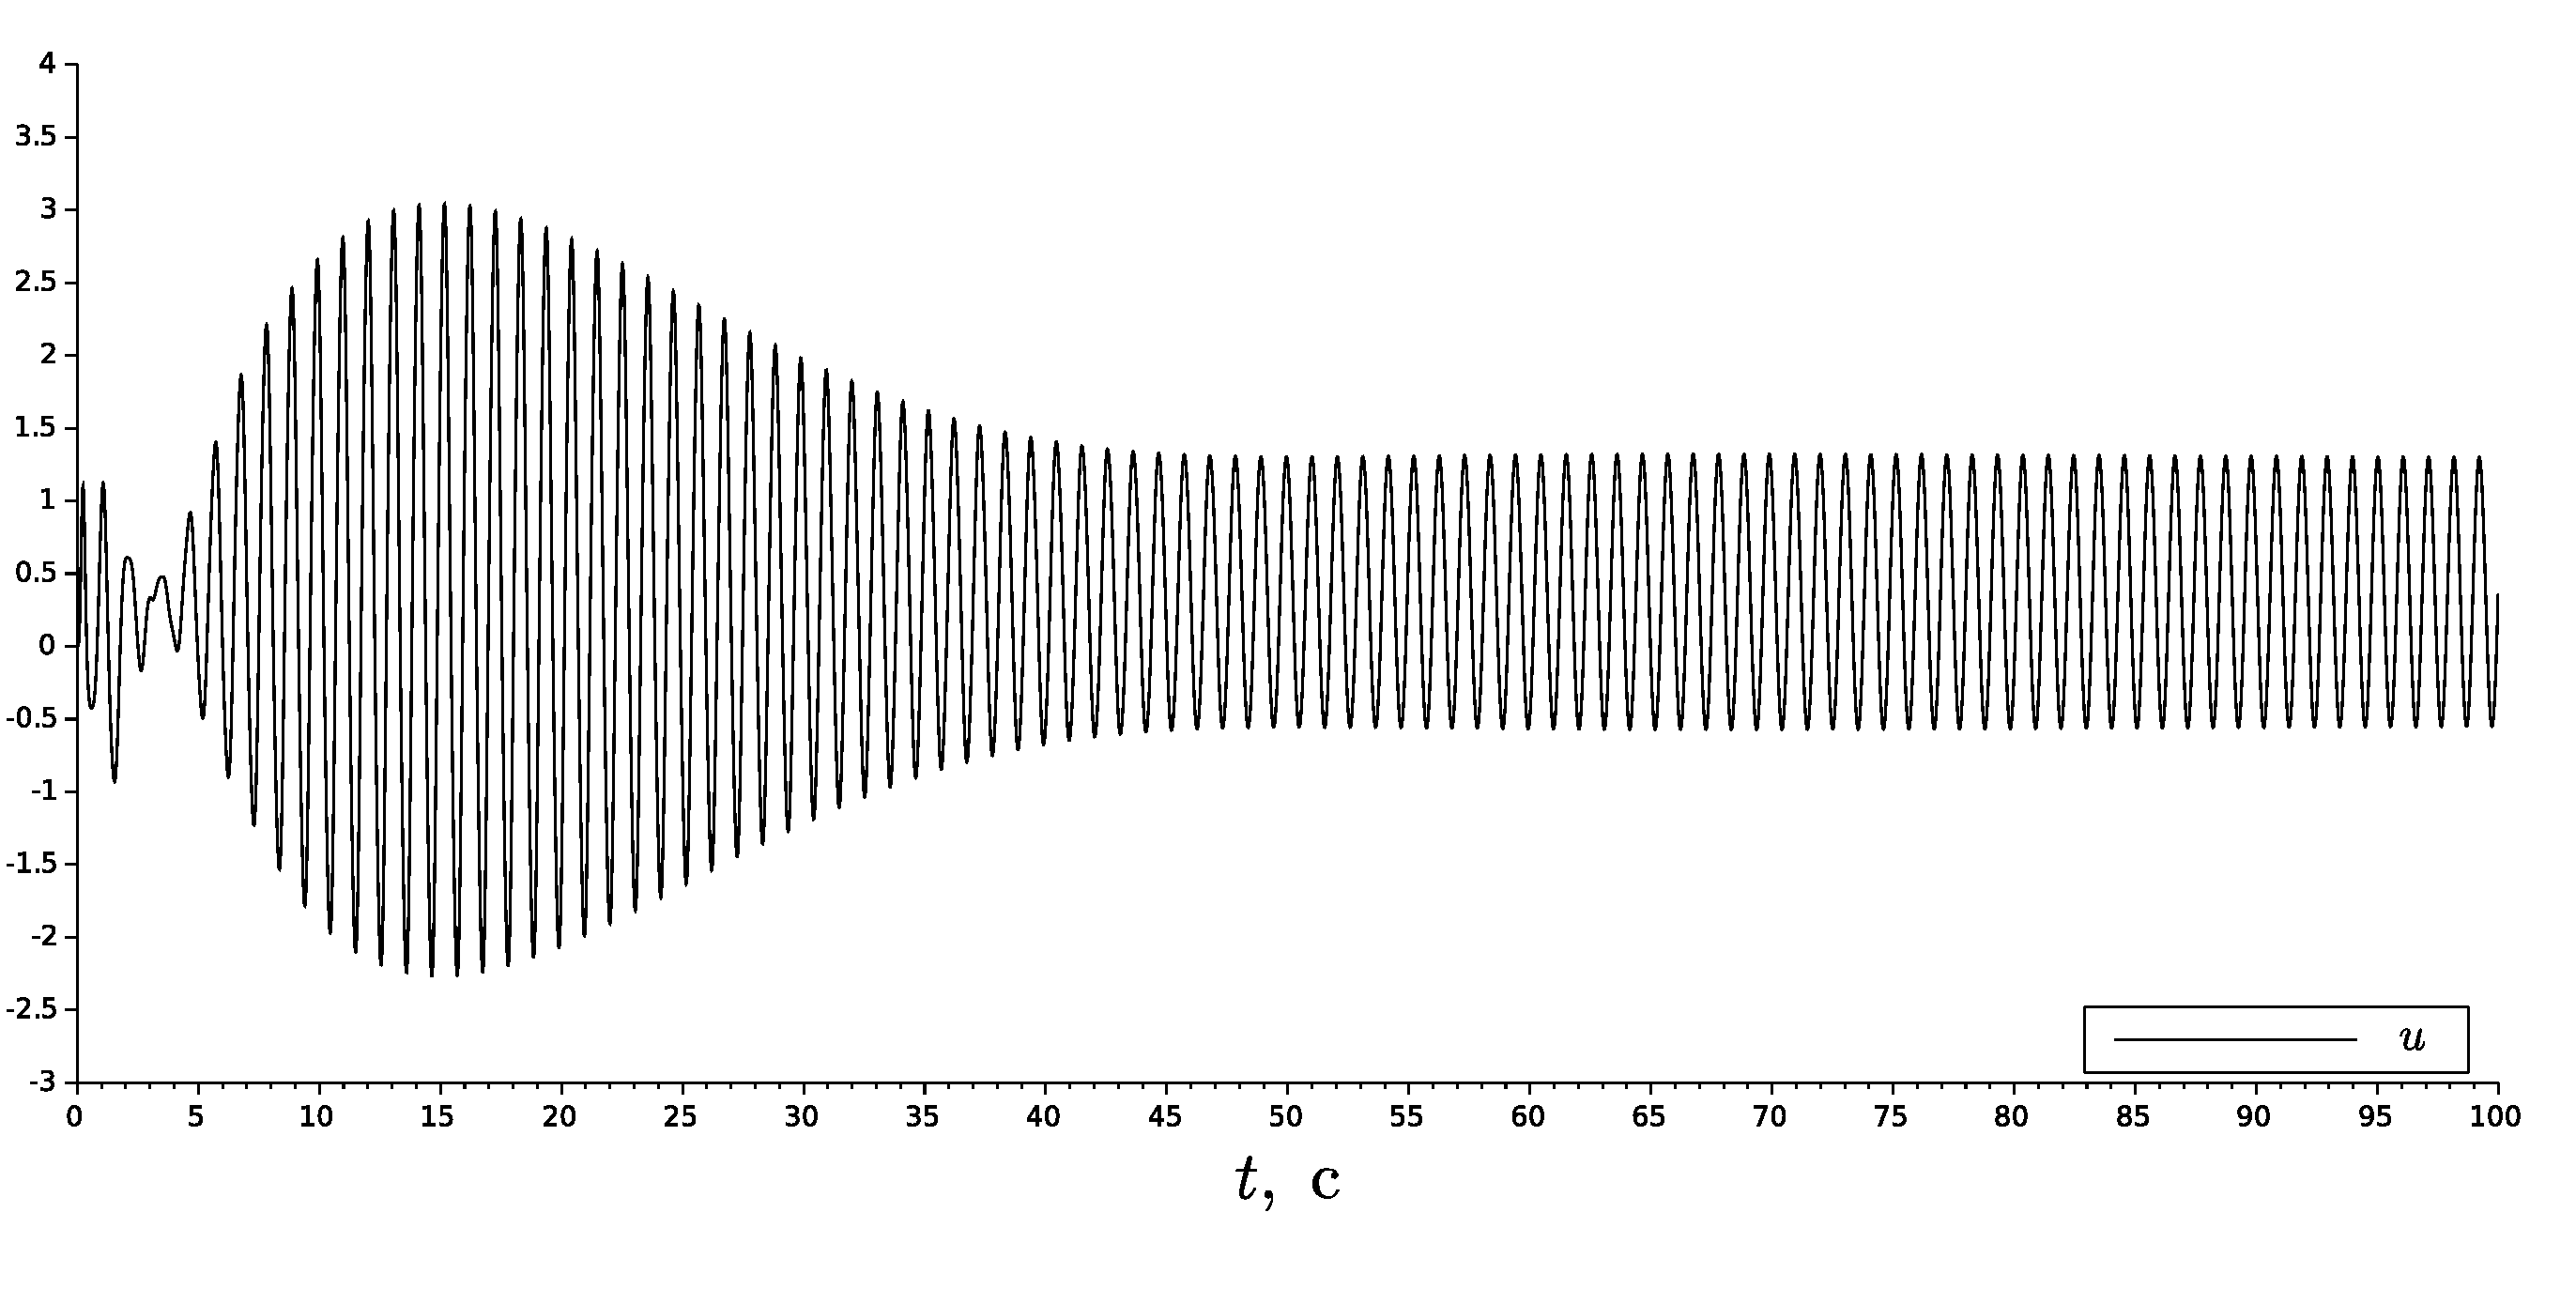
\includegraphics[width=\textwidth]{u.pdf}
	\caption{Управляющее воздействие $u$}
	\label{fg:fin_2}
\end{figure}

\clearpage
\begin{figure}[h!]
	\centering
	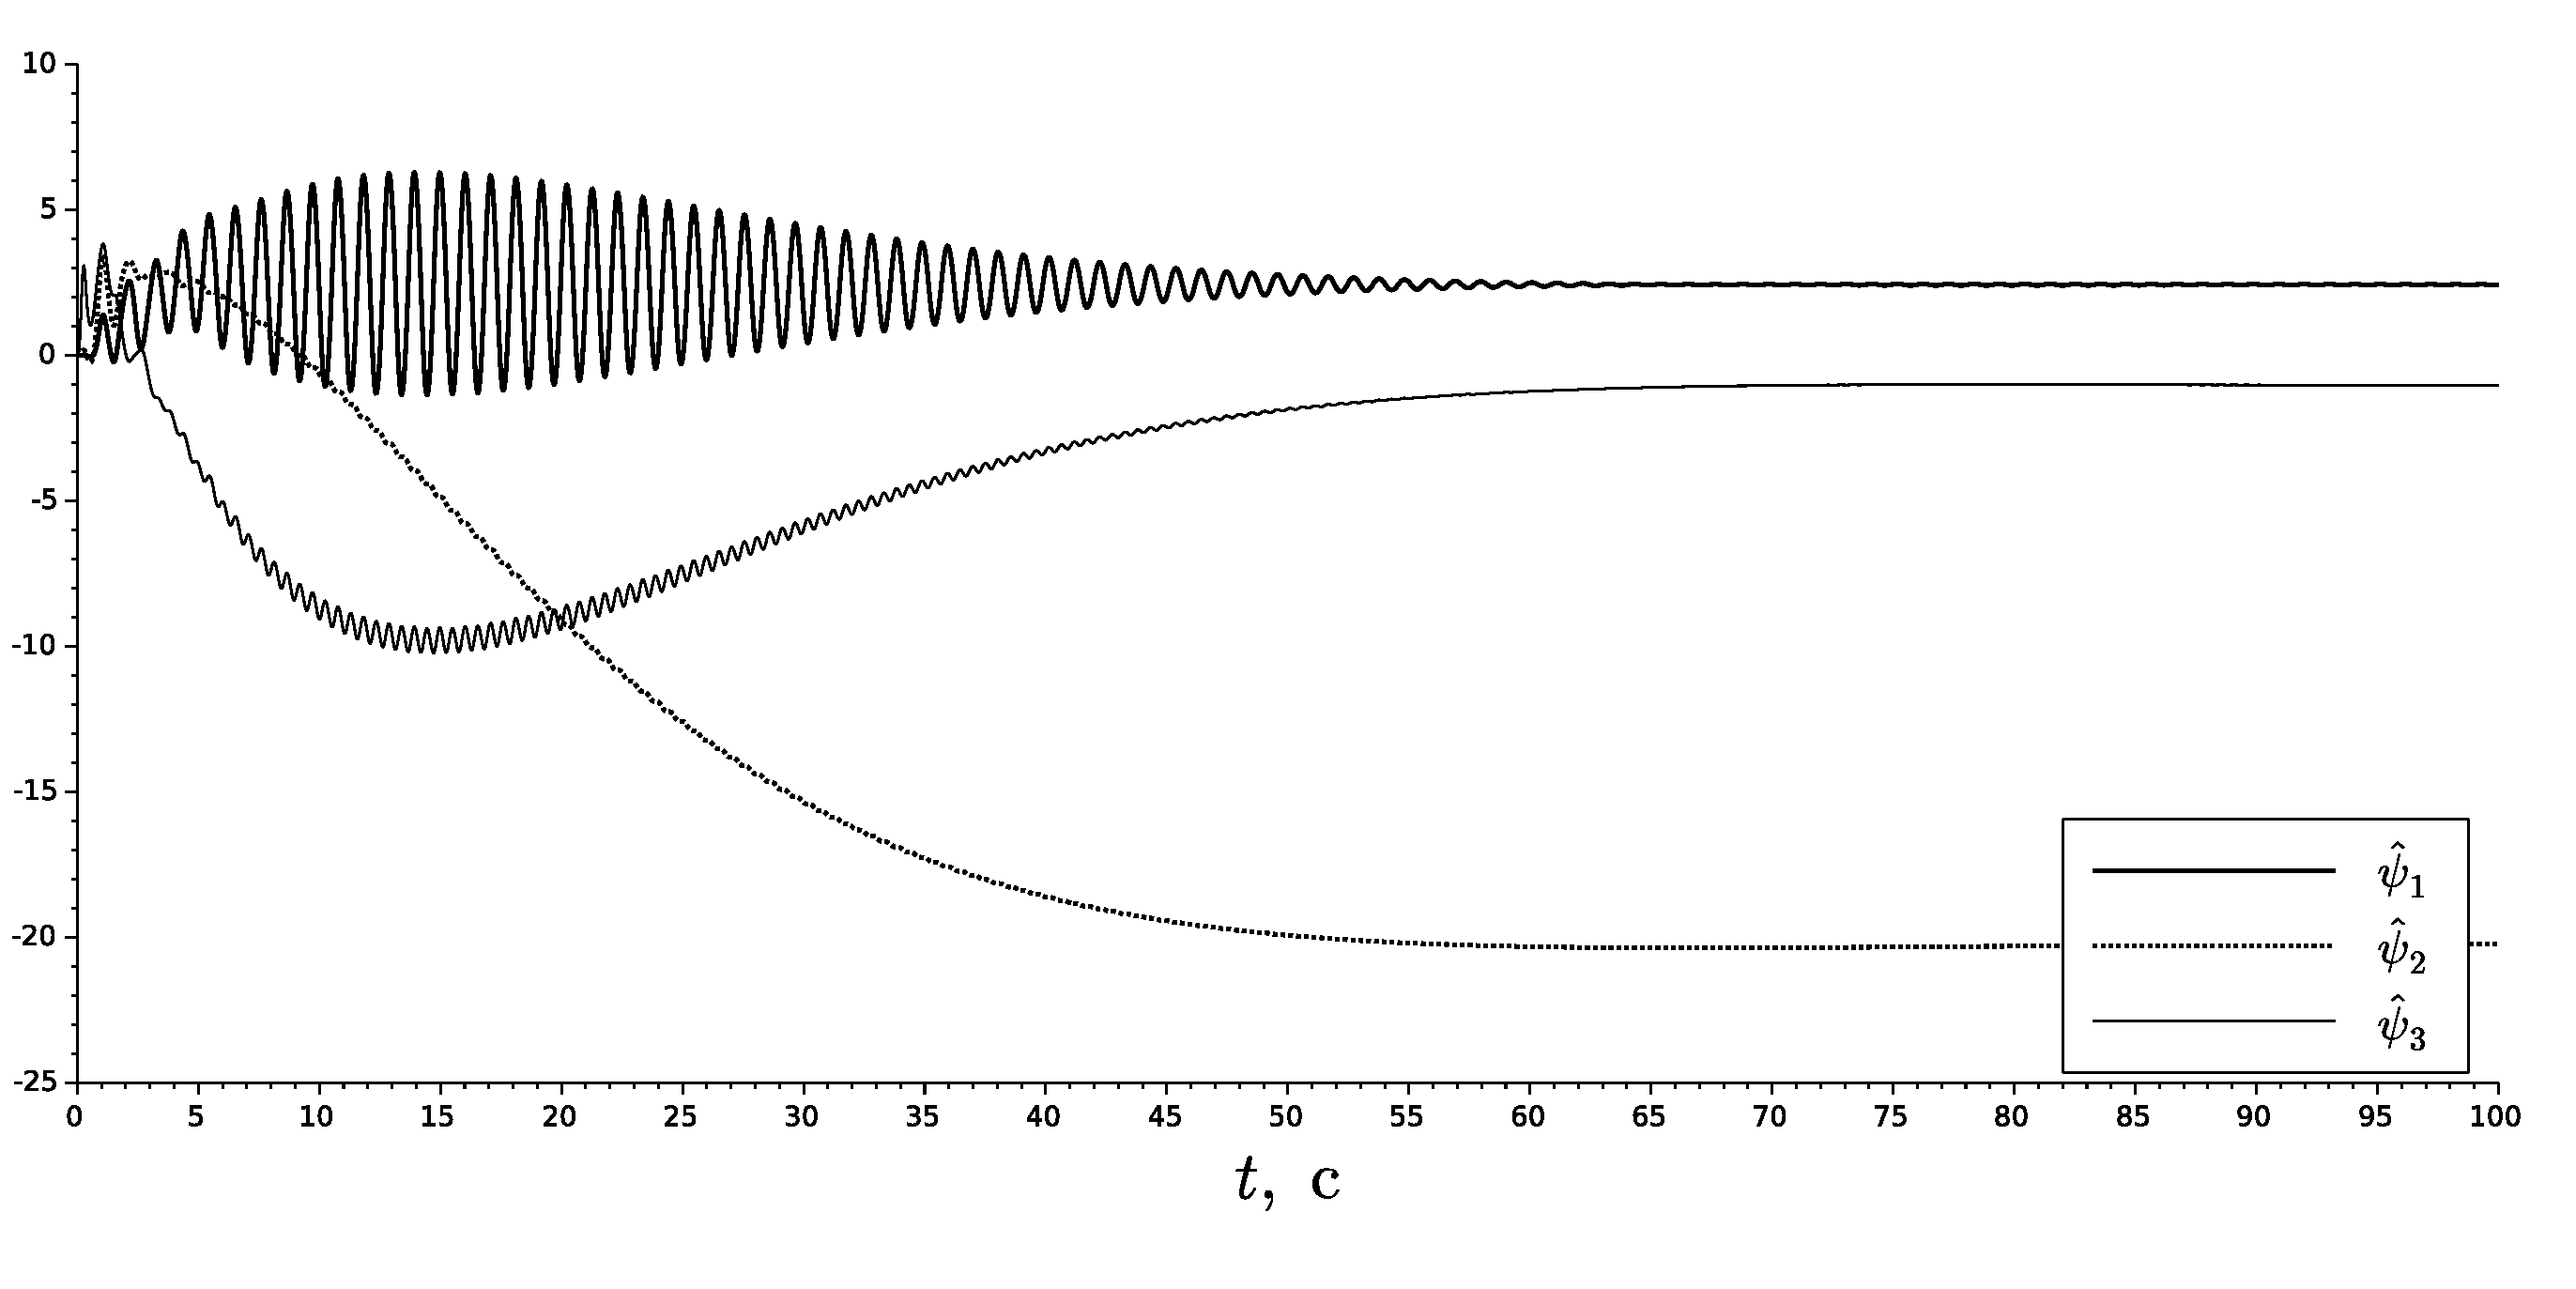
\includegraphics[width=\textwidth]{psi.pdf}
	\caption{Оценки параметров настраиваемого регулятора $\hat\psi$}
	\label{fg:fin_3}
\end{figure}


\section{Выводы по работе}
В~результате проделанной работы:
\begin{itemize}
	\item были проанализированы свойства заданного объекта управления и синтезировано стабилизирующее управления; 
	\item построена параметризованная модель генератора задающих воздействий относительно выходной переменной и адаптивный идентификатор его параметров;
	\item реализован адаптивный алгоритм слежения за неизвестным сигналом.
\end{itemize}

Из моделирование полученной системы слежения, представленного на рисунках~\ref{fg:generator_parametric_adapt_sh} - \ref{fg:fin_3}, видно, что после настройки регулятора, система удовлетворяет цели управления~\eqref{goal}.
